\documentclass[a4paper,12pt, oneside]{book}

%\usepackage{fullpage}
\usepackage[italian]{babel}
\usepackage[utf8]{inputenc}
\usepackage{amssymb}
\usepackage{amsthm}
\usepackage{graphics}
\usepackage{amsfonts}
\usepackage{listings}
\usepackage{amsmath}
\usepackage{amstext}
\usepackage{engrec}
\usepackage{rotating}
\usepackage[safe,extra]{tipa}
\usepackage{showkeys}
\usepackage{multirow}
\usepackage{hyperref}
\usepackage{microtype}
\usepackage{enumerate}
\usepackage{braket}
\usepackage{marginnote}
\usepackage{pgfplots}
\usepackage{cancel}
\usepackage{polynom}
\usepackage{booktabs}
\usepackage{enumitem}
\usepackage{framed}
\usepackage{pdfpages}
\usepackage{pgfplots}
\usepackage[cache=false]{minted}

\usepackage{tikz}\usetikzlibrary{er}\tikzset{multi  attribute /.style={attribute ,double  distance =1.5pt}}\tikzset{derived  attribute /.style={attribute ,dashed}}\tikzset{total /.style={double  distance =1.5pt}}\tikzset{every  entity /.style={draw=orange , fill=orange!20}}\tikzset{every  attribute /.style={draw=MediumPurple1, fill=MediumPurple1!20}}\tikzset{every  relationship /.style={draw=Chartreuse2, fill=Chartreuse2!20}}\newcommand{\key}[1]{\underline{#1}}

\usepackage{fancyhdr}
\pagestyle{fancy}
\fancyhead[LE,RO]{\slshape \rightmark}
\fancyhead[LO,RE]{\slshape \leftmark}
\fancyfoot[C]{\thepage}



\title{Basi di Dati}
\author{UniShare\\\\Davide Cozzi\\\href{https://t.me/dlcgold}{@dlcgold}\\\\Gabriele De Rosa\\\href{https://t.me/derogab}{@derogab} \\\\Federica Di Lauro\\\href{https://t.me/f_dila}{@f\textunderscore dila}}
\date{}

\pgfplotsset{compat=1.13}
\begin{document}
\maketitle

\definecolor{shadecolor}{gray}{0.80}
\setlist{leftmargin = 2cm}
\newtheorem{teorema}{Teorema}
\newtheorem{definizione}{Definizione}
\newtheorem{esempio}{Esempio}
\newtheorem{corollario}{Corollario}
\newtheorem{lemma}{Lemma}
\newtheorem{osservazione}{Osservazione}
\newtheorem{nota}{Nota}
\newtheorem{esercizio}{Esercizio}
\tableofcontents
\renewcommand{\chaptermark}[1]{%
	\markboth{\chaptername
		\ \thechapter.\ #1}{}}
\renewcommand{\sectionmark}[1]{\markright{\thesection.\ #1}}
\chapter{Introduzione}
\textbf{Questi appunti sono presi a ldurante le esercitazioni in laboratorio. Per quanto sia stata fatta una revisione è altamente probabile (praticamente certo) che possano contenere errori, sia di stampa che di vero e proprio contenuto. Per eventuali proposte di correzione effettuare una pull request. Link: } \url{https://github.com/dlcgold/Appunti}.\\
\textbf{Grazie mille e buono studio!}
\chapter{Introduzione al Corso}
Il corso di Basi di Dati affronta gli aspetti e i metodi per lo sviluppo di un database in maniera efficiente,
aspetto fondamentale per un informatico e per lo sviluppo ottimale di software. \newline
Il corso si divide in 7 parti:
\begin{enumerate}
	\item introduzione generale
	\item metodologie e modelli per il progetto delle basi di dati
	\item progettazione concettuale
	\item modello razionale
	\item progettazione logica
	\item linguaggio SQL
	\item algebra relazionale
\end{enumerate}
Le \textbf{informazioni} fanno parte delle risorse di un'azienda, soprattuto negli ultimi anni di clima globale,
per cui la gestione efficiente ed ottimale dei dati è fondamentale, come ad esempio Facebook ed Amazon fanno ampio
uso dei nostri dati, sia a scopi pubblicitari sia a scopi di marketing.

Un sistema informativo è una componente di un'organizzazione che gestiste le informazioni d'interesse, non per forza attraverso
un'automatizzazione e/o supporto di un calcolatore, infatti sin dall'antichita le banche
tenevano traccia dei depositi tramite un archivio cartaceo.

Una porzione automatizzate del sistema informativo si chiama sistema informatico, che si divide in:
\begin{itemize}
	\item acquisizione e memorizzazione
	\item aggiornamento
	\item interrogazione
	\item elaborazione
\end{itemize}
Le informazioni vengono gestite in vari modi, attraverso il linguaggio naturale, graficamente con schemi e/o numeri,
con il tempo si è arrivati a codifiche standard per quasi tutte le tipologie di informazioni, e sono rappresentate
nei sistemi informatici dai \emph{dati}, la cui differenza è che i dati sono valori senza alcun valore
mentre le informazioni stabilisce un'interpretazione attribuendo una semantica ai valori.

I dati sono una risorsa strategica in quanto sono stabili nel tempo, infatti solitamente i dati sono immutati
durante una migrazione tra un sistema e un altro, per questo lo sviluppo progettazione di un database rimane stabile in teoria,
senza notevoli cambiamenti durante la durata di un sistema informativo.

Un \textbf{Data Base} è una collezione di dati usati per rappresentare le informazioni di interesse di un sistema informativo,
definite solo una volta a cui un insieme di applicazioni ed utenti può accedere ad essi,
mentre un \textbf{DBMS} è un software per la gestione di un database.

I dati presenti in un database sono molti, indipendenti dal programma in cui vengono utilizzati e cui si cerca di evitare
la ridondanza, per garantire la consistenza delle informazioni.

Per la creazione di un database, al fine di garantire privatezza, affidabilità, efficienza ed efficacia,
sono presenti le seguenti tre fasi:
\begin{enumerate}
	\item definizione
	\item creazione e popolazione
	\item manipolazione
\end{enumerate}
Un organizzazione è divisa in vari settori e ogni settore ha un suo sottosistema informativo, non necessariamente disgiunto,
e i database solitamente sono condivisi, al fine di ridurre la ridonzanza delle informazioni, per cui sono presenti
meccanismi di autorizzazione e di controllo della concorrenza.\newline
Un database deve essere conservato a lungo termine e si ha una gestione delle \textbf{transazioni}:
insieme di operazioni da considerare indivisibile, atomico, corretto anche in presenza di concorrenza e con effetti definitivi.

La sequenza di operazioni nel database deve essere eseguita nella sua interezza, per cui l'effetto di
transazioni concorrenti deve essere coerente, infatti la conclusione positiva di una transazioni corrisponde ad un impegno,
\emph{commit}, a mantenere traccia del risultato, anche in presenza di guasti e di esecuzioni concorrente.\newline
Come tutti i software, i DBMS devono essere efficienti, utilizzando al meglio memoria e tempo, efficaci e produttivi.

Si hanno delle caratteristiche nell'approccio alla base dati:
\begin{itemize}
	\item natura autodescrittiva di un sistema di basi di dati: il sistema di basi di dati memorizza i dati con
	      anche una descrizionie completa della sua struttura(metadati), per consentire ai DBMS di lavorare con qualsiasi applicazione.
	\item separazione tra programmi e dati, infatti è possibile cambiare la struttura dati senza cambiare i programmi.
	\item astrazione dei dati: si usa un modello dati per nascondere dettagli e presentare
	      all'utente una visione concettuale del database.
	\item supporto di viste multiple dei dati, per cui ogni utente può usare una vista (view) differente del
	      database, contenente solo i dati di interesse per quell'utente.
	\item condivisione dei dati e gestione delle transazioni con utenti multipli.
\end{itemize}
I DBMS estendono le funzionalità dei file system, fornendo più servizi ed in maniera integrata.

In ogni base di dati si ha:
\begin{itemize}
	\item lo \textbf{schema}, sostanzialmente invariante nel tempo, che ne descrive la struttura, l'aspetto intensionale.
	\item l'\textbf{istanza}, i valori attuali, che possono cambiare anche molto rapidamente, l'aspetto estensionale "concreto".
\end{itemize}
Per lo sviluppo delle basi di dati si hanno due tipi di modelli, ambedue importanti:
\begin{itemize}
	\item \textbf{modelli logici}, adottati nei DBMS esistenti per l'organizzazione dei dati,
	      utilizzati dai programmi e sono indipendenti dalle strutture fisiche
	\item \textbf{modelli concettuali} che permettono di rappresentare i dati in modo indipendente da ogni sistema,
	      con il fine di descrivere i concetti del mondo reali;sono usati nelle fasi preliminari di progettazione
	      e il più diffuso è il modello \textbf{Entity-Relationship}.
\end{itemize}
%immagine architettura standard
Un database è organizzato solitamente attraverso i tre schemi dell'architettura ANSI/SPARC:
\begin{enumerate}
	\item [schema logico:] descrizione dell'intera base di dati nel modello logico “principale” del DBMS,
	      ossia si definisce la struttura concettuale del database,
	      senza considerare l'implementazione fisica nel DBMS.
	\item [schema fisico:] rappresentazione dello schema logico per mezzo di strutture fisiche di memorizzazione
	\item [schema esterno:] descrizione di parte della base di dati in un modello logico
	      (“viste” parziali, derivate, anche in modelli diversi)
\end{enumerate}
L'accesso ai dati avviene solo mediante il livello esterno, il quale a volte coincide con quello logico,
e si hanno 2 forme di indipendenza: quella fisica, in cui è possibile interagire con il DBMS senza conoscere la struttura fisica
e quella logica, in cui si può accedere al livello esterno senza interagire con lo schema logico.

Per la definizione dei database ci sono quattro tipologie di linguaggi:
\begin{itemize}
	\item \textbf{DLL}(Data Manipulation Languages) linguaggio per definire i dati
	\item \textbf{DML}(Data Manipulation Languages) linguaggio per la manipolazione dei dati
	\item \textbf{DCL}(Data Control Languages) linguaggio per il controllo degli accessi al database
	\item \textbf{DQL}(Data Query Languages) linguaggio per effettuare delle interrogazioni al database
\end{itemize}
Noi vedremo SQL per definire i database, linguaggio basato sull'algebra relazionale che implementa tutti e 4 le tipologie
di linguaggi per la gestione di un database.

Si hanno due tipi di utenti:
\begin{enumerate}
	\item \textbf{utenti finali (terminalisti):} eseguono applicazioni predefinite (transazioni)
	\item \textbf{utenti casuali:} eseguono operazioni non previste a priori, usando linguaggi interattivi
\end{enumerate}
inoltre si hanno:
\begin{itemize}
	\item progettisti e realizzatori di DBMS
	\item progettisti della base di dati e amministratori della base di dati (DBA),
	      persona o gruppo di persone responsabile del controllo centralizzato del database,
	      in tutti i suoi aspetti.
	\item progettisti e programmatori di applicazioni
\end{itemize}
\begin{center}
	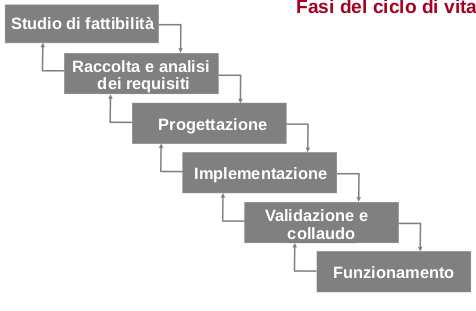
\includegraphics[scale=0.8]{img/bas.png}
\end{center}
Come visto anche nel corso di analisi e progettazione del software e nella figura X,
durante lo sviluppo di un sistema informatico si hanno le seguente fasi:
\begin{itemize}
	\item \textbf{studio di fattibilità}, definizione di costi, priorità e competenze per un progetto
	\item\textbf{raccolta e analisi dei requisiti}, ovvero lo studio delle proprietà del sistema
	\item \textbf{progettazione} di dati e funzioni
	\item \textbf{implementazione}
	\item \textbf{validazione e collaudo},che comprendono anche test da parte del cliente
	\item \textbf{funzionamento}, ovvero lo stadio finale dove il sistema diventa effettivamente operativo
\end{itemize}
In questo corso ci occuperemo soltanto delle fasi di progettazione ed implementazione di base di dati,
lasciando l'analisi delle altre fasi al corso ed ai libri di Ingegneria del Software.\newline
In questo processo a rimanere stabili sono prettamente i \textbf{dati} infatti prima si progetta la base dati,
con una \textbf{metodologia di progetto}, e poi il software.
\begin{center}
	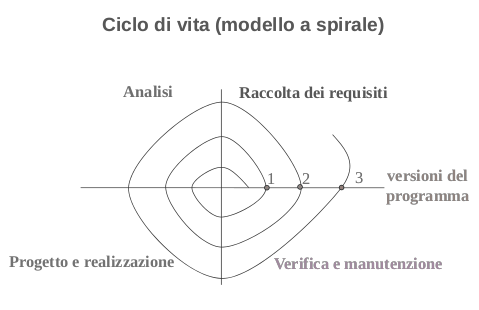
\includegraphics[scale=2.8]{img/bas2.png}
\end{center}
Una \textbf{metodologia} è un'articolazione in fasi di guida ad un'attività di progettazione, in caso
di una base dati la metodologia, con il fine di separare il cosa rappresentare dal come, è la seguente:
\begin{itemize}
	\item suddivida la progettazione in fasi indipendenti
	\item fornisca strategie e criteri di scelta in caso di alternative
	\item fornisca modelli di riferimento (i linguaggi)
	\item garantisca generalità rispetto al problema
	\item garantisca qualità e facilità d'uso
\end{itemize}
\begin{center}
	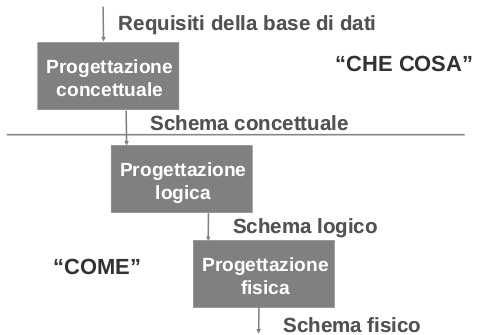
\includegraphics[scale=2.5]{img/bas3.png}
\end{center}
\begin{center}
	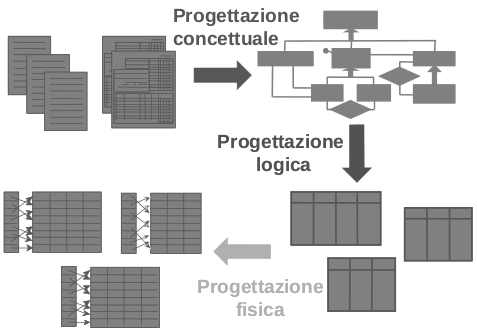
\includegraphics[scale=2.5]{img/bas4.png}
\end{center}
Come si può notare nella figura X1, la metodologia corrente di modellazione di un database
prevede la definizione e l'esecuzione delle seguenti fasi:
\begin{itemize}
	\item la \textbf{progettazione concettuale} consiste nel tradurre i requisiti del sistema informatico
	      in una descrizione formale, integrata e indipendente dalle scelte implementative (DBMS, SW e HW)
	\item la \textbf{progettazione concettuale} consiste nella traduzione dello schema concettuale nel modello dei dati
	      scelto per la modellazione, ottenendo uno schema logico, espresso nel DDL del DBMS.\newline
	      In questa fase si considerano anche aspetti legati ai vincoli ed all'efficienza. Si hanno due sotto-fasi:
	      \begin{itemize}
		      \item ristrutturazione dello schema concettuale
		      \item traduzione verso il modello logico
	      \end{itemize}
	\item la \textbf{progettazione fisica} completa lo schema logico ottenuto con le specifiche proprie del DBMS scelto.
	      Il risultato è lo schema fisico che descrive le strutture di memorizzazione ed accesso ai dati
\end{itemize}
Incominciamo nel prossimo capitolo a considerare la progettazione concettuale, per poi analizzare nei successivi capitolo
in dettaglio anche la fase di progettazione concettuale e il linguaggio SQL.

\chapter{Progettazione Concettuale:ER}
Come abbiamo già introdotto nel precedente capitolo, affrontiamo ora la progettazione concettuale di una base dati attraverso
il modello \textbf{ER}(Entity Relationships), modello concettuale che fornisce una serie di strutture
atte a descrivere in maniera semplice e facile la realtà di interesse da modellare.

Si hanno dei vantaggi con la progettazione concettuale, prevale infatti l'aspetto intensionale indipendente
dalla tecnologia ed è una rappresentazione grafica ed è utile per la documentazione, in quanto facilmente comprensibile anche
da persone poco avezze alla tecnologia e ai database.

In uno schema ER si hanno i seguenti costrutti, come si nota nella figura Y,
la cui rappresentazione effettiva varia in quanto vi sono più versioni di ER:
\begin{itemize}
	\item \textbf{entità}: classe di oggetti con proprietà comune ed esistenza "autonoma", della quale si vogliono specificare
	      fatti specifici;ogni entità ha un nome univoco, espressivo e al singolare.
	\item \textbf{relazione}: rappresentano legami logici, significativi per la realtà da modellare, tra due o più entità.\newline
	      Un'occorrenza di relazione è un n-upla costituita da occorrenze di entità, una per ciascuna delle entità coinvolte,
	      e ogni relazione ha un nome univoco, in cui è preferibile assegnare un sostantivo per evitare di stabilire un verso alla relazione.\\
	      Essendo una relazione matematica tra le entità coinvolte non è possibile avere delle n-uple identiche, con conseguenze
	      per la realtà da rappresentare, per esempio non è possibile attraverso una relazione il fatto che è possibile
	      ripetere un esame, obbligando a rappresentare l'esame come entità e non più come relazione.
	\item \textbf{attributo semplice}: associa ad ogni istanza di entità o associazione un valore, definito su un dominio di valori,
	      specificato nella documentazione associata, con il fine di descrivere le proprietà elementari
	      di entità e/o relazioni disegnate per rappresentare la realtà d'interesse.\newline
	\item \textbf{attributo composto}: raggruppamento di attributi di una medesima entità/relazione con affinità di significato e/o uso
	      come ad esempio possiamo raggruppare gli attributi Via, Numero Civico e Cap dall'entità persona per formare
	      l'attributo composto Indirizzo.
	\item \textbf{cardinalità delle relazioni}: vengono specificate per ogni relazione e descrivono il numero minimo e massimo di occorrenze
	      di relazione, a cui una occorrenza dell'entità può partecipare alla relazione, ossia quante volte un'occorrenza
	      di un'entità può essere legata ad occorrenze delle altre entità coinvolte.\newline
	      È possibile assegnare un qualunque intero non negativo, con l'unico vincolo che la cardinalità minima
	      sia minore o uguale alla cardinalità massima e di solito si usano i valori $0, 1 \text{e} N$, indicanti
	      zero, una o molte occorrenze, senza preoccuparsi in caso di $N$ del numero effettivo di occorrenze.
	\item \textbf{cardinalità di un attributo}: descrivono il numero minimo e massimo di valori dell'attributo
	      associati all'entità e/o relazione, con la cardinalità $(1, 1)$ stabilita come default,
	      che può essere vista come funzione che associa ad ogni occorenza di entitò un solo valore dell'attributo;
	      si hanno le stesse consetutidini delle cardinalità delle relazioni.
	\item \textbf{identificatore interno}: permette di identificare in maniera univoca un'entità ed un identificatore è interno
	      in caso sia uno o più attributi di un'entità, tutti con cardinalità $(1, 1)$.
	\item \textbf{identificatore esterno}: un identificatore è esterno, in caso un'entità $E$  viene identificata da un'attributo
	      di un'entità $F$, cui esiste una relazione uno a uno tra l'entità $E$ e $F$.\newline
	      È possibile, anche se molto raro, avere la definizione dell'identificatore usando entità di entità, ossia
	      l'identificatore dell'entità $E$ viene definito nell'entità $G$, cui esiste una relazione con l'entità $F$
	      che a sua volta ha una relazione con l'entità $E$, ma si può capire da quanto è contorto il ragionamento
	      qual'è la sua percentale d'utilizzo nella modellazione dello schema ER.
	\item \textbf{generalizzazione}: rappresentano legami logici tra un entità $E$, detta padre, e una serie di entità $E_1, E_2, \dots, E_n$,
	      dette figlie, di cui l'entità $E$ rappresenta un caso generale della serie di entità figlie.\newline
	      Tra le entità coinvolte in una generalizzazione valgono le seguenti proprietà:
	      \begin{itemize}
		      \item ogni occorrenza di un'entità figlia è anche un'occorrenza dell'entità genitore.
		      \item ogni proprietà dell'entità genitore è anche una proprietà delle entità figlie, quindi
		            nello schema ER non devono essere rappresentate, e ciò prende il nome di ereditarietà.
	      \end{itemize}
	      Le generalizzazioni possono essere classificate sulla base di due proprietà ortogonali:
	      \begin{itemize}
		      \item una generalizzazione è totale se ogni occorrenza del genitore è un occorrenza di almeno
		            uno dei figli, altrimenti è parziale.
		      \item una generalizzazione è esclusiva se ogni occorrenza del genitore è al più un'occorrenza
		            di una delle entità figlie, altrimenti è sovrrapposta.
	      \end{itemize}
	\item \textbf{sottoinsieme}: generalizzazione con soltanto un entità figlia, di cui solitamente rappresenta una parte
	      dell'entità genitore come ad esempio gli studenti sono un sottoinsieme delle persone.
\end{itemize}

\begin{figure}
	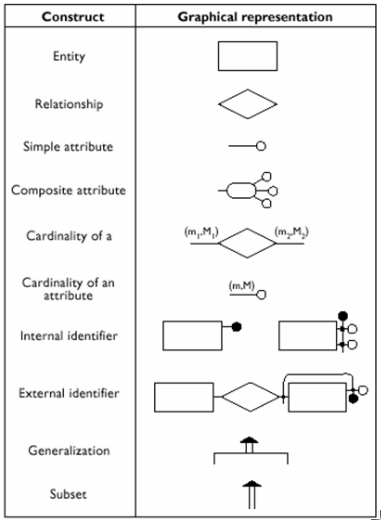
\includegraphics[scale=0.8]{img/bas6.png}
\end{figure}
Un'occorrenza, o istanza, di un'entità, è un oggetto della classe che l'entità rappresenta,
ma noi rappresentiamo le entità dello schema concettuale non le singole istanze, in quanto esse
sono variabili nel tempo a differenza della struttura, concetto fondamentale per definire un modello funzionale.

Nessuno impone un tipo per un certo attributo, possono essere anche complessi di cui però non ci interessano le informazioni
che lo rappresentano, come ad esempio una foto può essere un attributo, ma se ho bisogno dell'autore della foto,
non sarà più un attributo ma un'altra entità.

Un'\textbf{istanza di associazione} è una combinazione o aggregazione di istanze di entità che prendono
parte all'associazione (per esempio "prof. Schettini" è istanza di associazione per l'entità docente).\newline
Le relazioni possono avere attributi, con valori specificati in un certo dominio, che  modella una proprietà del legame
tra tutte le entità rappresentato dalla relazione.

Una associazione può coinvolgere “due o più volte” la stessa entità e ciò si chiama \emph{associazione ricorsiva o ad anello},
come si nota nella figura XXXX, ed è molto utile per definire le relazioni subordinazione e/o comunicazioni tra istanze
di una stessa entità, come nel caso della relazione sovrano, indicante la lista dei sovrani con i predecessori e successori;
in queste associazioni è necessario aggiungere la specifica dei \textbf{ruoli}, come nell'esempio SDERR, per specificare
in maniera chiara e non ambigua quale è il verso della relazione.

Un'associazione ad anello, ovviamente essendo una relazione, può avere delle proprietà come ad esempio la relazione della figura
SJDFHJF è irriflessiva, intransitiva e asimetrica.

\begin{figure}
	\centering
	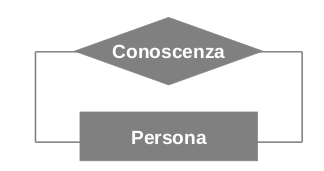
\includegraphics[scale=2.5]{img/bas7.png}
\end{figure}

\begin{center}
	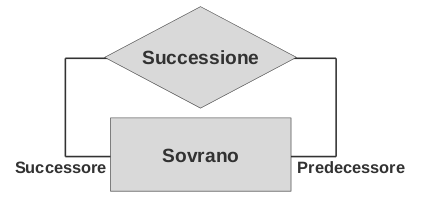
\includegraphics[scale=2.5]{img/bas8.png}
\end{center}

\newpage
\textit{Descrivere lo schema concettuale della seguente
	realtà:
	I docenti hanno un codice fiscale ed una età. I
	docenti operano nei corsi di laurea (si dice che
	afferiscono ai corsi di laurea). Interessa la data di
	afferenza dei docenti ai corsi di laurea. I corsi di
	laurea hanno un codice ed un nome, ed
	appartengono alle facoltà. Ogni facoltà ha un nome}
\begin{center}
	\begin{tikzpicture}[node  distance =7em]
		\node[entity] (docente) {docente};
		\node[attribute] (età) [above left of =  docente] {età} edge (docente);
		\node[attribute] (codice) [above of = docente] {codice fiscale} edge (docente);
		\node[relationship] (operatore) [right of = docente] {operatore} edge (docente);
		\node[attribute] (data) [below of = operatore ] {data} edge (operatore);
		\node [entity] (laurea) [right of = operatore] {laurea} edge (operatore);
		\node[attribute] (cod) [above of =  laurea] {nome} edge (laurea);
		\node[attribute] (nome) [above right of = laurea] {codice} edge (laurea);
		\node[relationship] (appartenenza) [below of = laurea] {appartenenza} edge (laurea);
		\node [entity] (facoltà) [below of = appartenenza] {facoltà} edge (appartenenza);
		\node[attribute] (nomee) [below of = facoltà] {nome} edge (facoltà);
	\end{tikzpicture}
\end{center}
\newpage
\begin{esempio}
	Descrivere lo schema concettuale della seguente
	realtà:
	Degli impiegati interessa il codice fiscale, il nome, il
	cognome, i dipartimenti ai quali afferiscono (con la
	data di afferenza), ed i progetti ai quali partecipano.
	Dei progetti interessa il nome, il budget, e la città in
	cui hanno luogo le corrispondenti attività. Alcuni
	progetti sono parti di altri progetti, e sono detti loro
	sottoprogetti. Dei dipartimenti interessa il nome, il
	numero di telefono, gli impiegati che li dirigono, e la
	città dove è localizzata la sede. Delle città interessa
	il nome e la regione:
	\begin{center}
		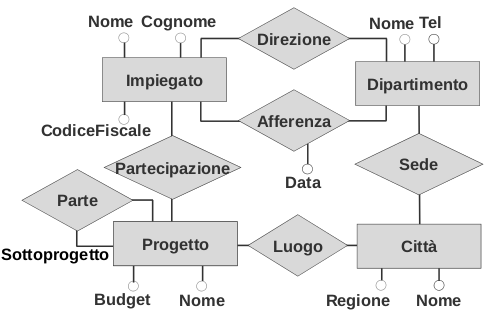
\includegraphics[scale=3]{img/er.png}
	\end{center}
\end{esempio}
Nella scelta del costrutto ideale, per rappresentare in maniera fedele e corretta la realtà, si usano le seguenti "regole":
\begin{itemize}
	\item \textbf{entità}: si usa un entità in caso vengano rispettate le seguenti proprietà:
	      le sue istanze sono significative indipendentemente dalle altre istanze, se si ha o si può avere delle proprietà
	      indipendenti dagli altri concetti oppure se il concetto da rappresentare è importante per la realtà da modellare.

	\item \textbf{attributo}: si usa un'attributo in caso succedono i seguenti avvenimenti: non ha senso
	      considerare una sua instanza a se stante ad altre instanze, le istanze non sono concettualmente significative
	      oppure serve soltanto rappresentare una proprietà locale di un altro concetto.

	\item \textbf{relazione}: si dovrebbe usare una relazione in caso non ha senso pensare alla partecipazione
	      delle sue instanze ad altre relazioni e le sue istanze non sono significative indipendentemente da altre istanze,
	      ossia una sua istanza ha senso se messa in relazione con altre istanze, provenienti da altri costrutti.

\end{itemize}

\begin{center}
	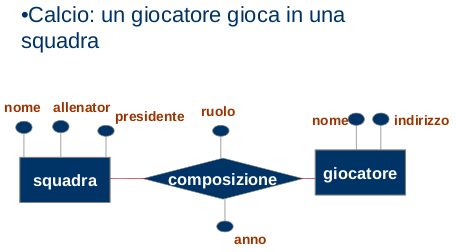
\includegraphics[scale=1]{img/er2.png}
\end{center}
\begin{esempio}
	\begin{itemize}
		\item ogni zoo è diviso in aree diverse a seconda che si tratti di rettili, pesci, uccelli, scimmie, grandi mammiferi, ... Ogni area è dotata di: nome,
		      indirizzo, dimensione, numero di sezioni.
		\item per ogni tipo di animale ci sono informazioni che riguardano: classificazione zoologica, nome comune (giraffa, elefante, serpente,
		      tartaruga, ...), habitat, alimentazione, ... Per ogni tipo di animale c'è un diverso veterinario specialista, dipendente dello zoo.
		\item ogni tipo di animale è rappresentato da esemplari e relativi dati anagrafici: nome proprio (giraffa Enrico, giraffa Giulia, ...), data di nascita,
		      Paese di provenienza, data di arrivo allo zoo, ...
		\item ogni esemplare è dotato di più schede sanitarie contenenti ognuna: la data della visita, referto, dieta, nome del veterinario, ...

	\end{itemize}
	\begin{center}
		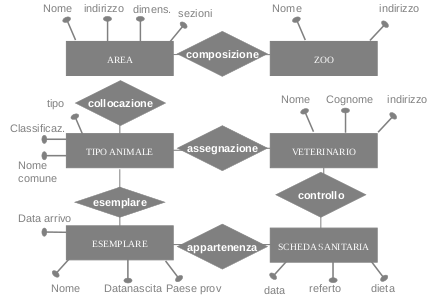
\includegraphics[scale=0.8]{img/er3.png}
	\end{center}
	lo zoo ha degli attributi che vanno indicati anche se non richiesti dalla traccia per evitare ambiguità. Dato che ogni scheda è collegata ad un veterinario, di cui ho un'entità la collego a veterinario con una relazione e non ne faccio  un attributo
\end{esempio}
\begin{center}
	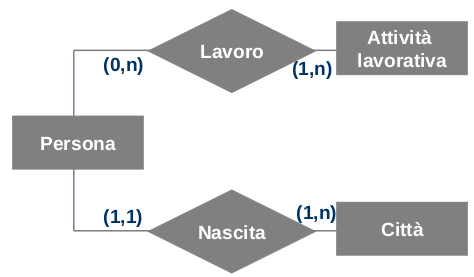
\includegraphics[scale=0.8]{img/er4.png}
\end{center}
\begin{center}
	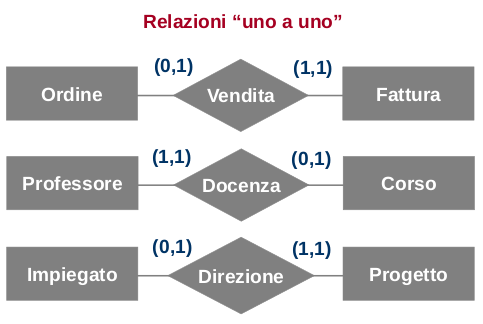
\includegraphics[scale=0.6]{img/er7.png}
\end{center}
\begin{center}
	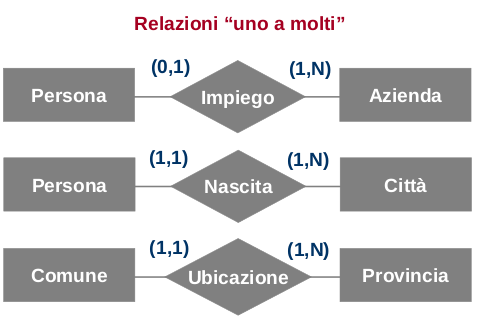
\includegraphics[scale=0.6]{img/er6.png}
\end{center}
\begin{center}
	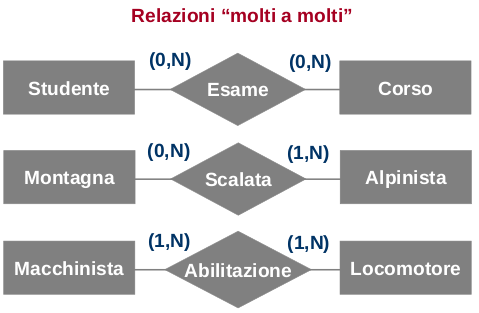
\includegraphics[scale=0.6]{img/er5.png}
\end{center}
vediamo un esempio:
\begin{esempio}
	si ha:
	\begin{center}
		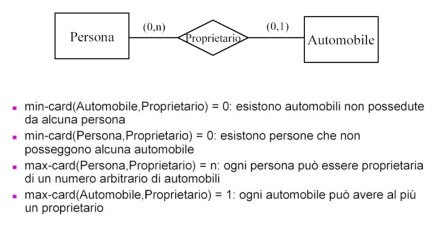
\includegraphics[scale=0.8]{img/er8.png}
	\end{center}

\end{esempio}
\begin{center}
	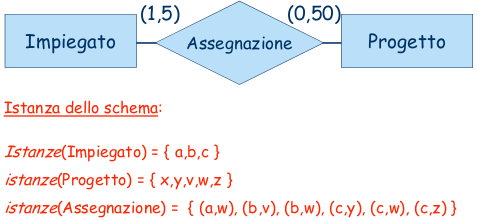
\includegraphics[scale=0.8]{img/er9.png}
\end{center}
\textit{Ad ogni impiegato sono assegnati da 1 a 5 progetti e ogni progetto è assegnato ad al più 50 impiegati. a,b,c compaiono in almeno una istanza di Assegnazione. x non compare nelle istanze di Assegnazione. Infine ci sono progetti (ad esempio lanciati da poco
	tempo) che possono non essere assegnati a nessun
	impiegato}\\
\begin{center}
	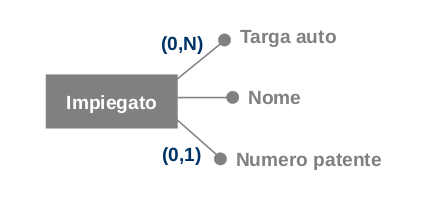
\includegraphics[scale=0.8]{img/er10.png}
\end{center}
\begin{center}
	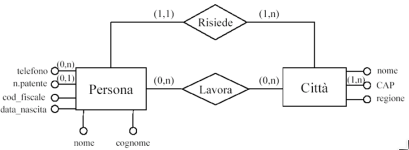
\includegraphics[scale=0.8]{img/er11.png}
\end{center}
\begin{center}
	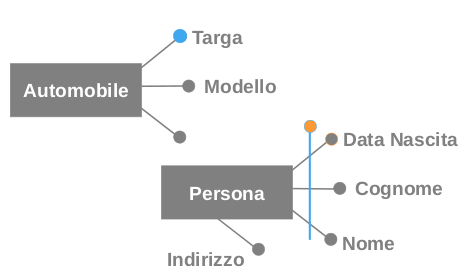
\includegraphics[scale=0.8]{img/er12.png}
\end{center}
\begin{center}
	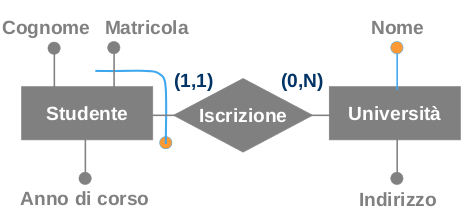
\includegraphics[scale=0.8]{img/er13.png}
\end{center}
vediamo un esempio complesso, che è preso da un vecchio esempio:
\begin{center}
	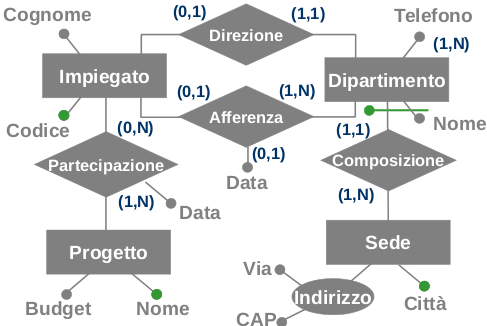
\includegraphics[scale=0.8]{img/er14.png}
\end{center}

\begin{center}
	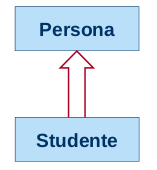
\includegraphics[scale=0.8]{img/isa.png}
\end{center}

\begin{center}
	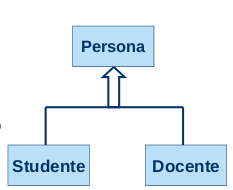
\includegraphics[scale=2.5]{img/isa3.png}
\end{center}
\begin{center}
	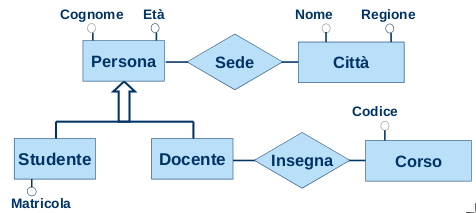
\includegraphics[scale=0.5]{img/isa4.png}
\end{center}
\begin{center}
	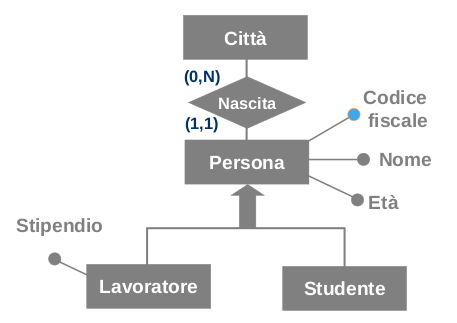
\includegraphics[scale=0.8]{img/isa5.png}
\end{center}
\begin{center}
	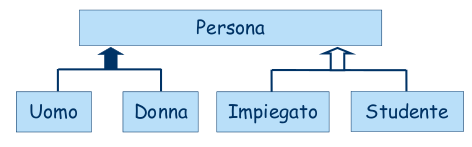
\includegraphics[scale=0.8]{img/isa6.png}
\end{center}
\begin{center}
	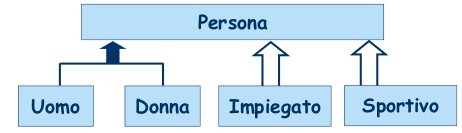
\includegraphics[scale=0.8]{img/isa7.png}
\end{center}
\begin{center}
	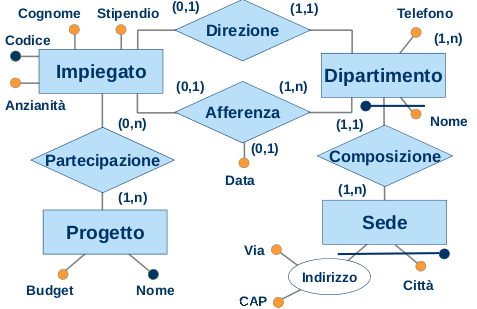
\includegraphics[scale=2.5]{img/vin.png}
\end{center}
\begin{center}
	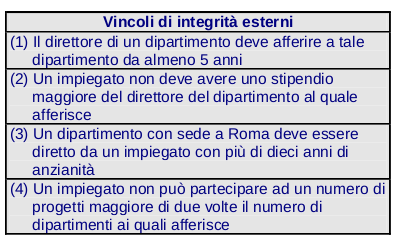
\includegraphics[scale=0.7]{img/vin2.png}
\end{center}
\begin{center}
	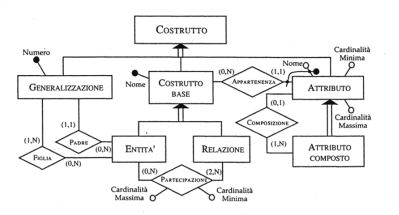
\includegraphics[scale=0.8]{img/vin3.png}
\end{center}

\chapter{Modello Relazionale}
Dopo aver introdotto il modello concettuale, specifichiamo ed analizziamo ora il modello logico necessario per
rappresentare in maniera efficace ed efficiente la base dati modellata.\newline
Analizziamo il modello relazionale, il più diffuso dei modelli dei dati, in cui si utilizzano le tabelle e le relazioni
per ottenere la rappresentazione voluta, introdotto negli anni '70 con l'obiettivo di rendere indipendenti i dati,
ossia separare la modellazione ``concettuale'' dall'effettiva implementazione fisica sul DBMS.

Il modello relazionale, presenta una notevole differenza dai modelli precedenti, dato che i riferimenti
fra dati in strutture diverse sono rappresentati per mezzo dei valori stessi, garantendo così l'indipendenza dei dati.

Il concetto di relazione, ovviamente proviene dalla teoria degli insiemi, rappresenta un sottoinsieme
del prodotto cartesiano ma nel modello relazionale si utilizza una variante di esso, ossia ad ogni dominio,
su cui è definito il prodotto cartesiano, viene associato un nome, chiamato \emph{attributo},
al fine di superare la struttura posizionale della relazione matematica.

Questo aspetto di utilizzare un'attributo con una notazione non posizionale ci garantisce di poter 
accedere ai campi di una tupla mediante un nome e soprattutto ci evita di stabilire un ordine tra 
i diversi campi, ad esempio chi stabilisce che la matricola sia prima del nome e non viceversa.

Forniamo ora un pò di formalismo al fine di definire in maniera non ambigua il concetto di base di dati:
\begin{definizione}
    Si definisce \emph{dominio} una funzione $dom:X \to D$ in cui si associa ogni attributo $A \in X$ un 
    dominio $dom(A) \in D$ mentre si definisce tupla su un insieme di attributi $X$ una funzione $t$ che
    associa ogni elemento di $X$ un elemento appartenente al dominio $dom(X)$.
\end{definizione}
\begin{definizione}
    Si definisce \emph{schema di relazione} $R(X)$ formato da $R$ indicante il nome della relazione mentre $X$
    indica un insieme di attributi, a cui ad ogni attributo viene associato un dominio, come abbiamo definito
    nella definizione precedente.\newline
    Si definisce invece \emph{istanza di relazione} su uno schema $R(X)$ è un insieme $r$ di tuple definite su
    $X$, a cui si può accedere ad un attributo della tupla attraverso $r.a$, con $a$ nome di un attributo.
\end{definizione}
\begin{definizione}
    Si definisce \emph{schema di base di dati} un insieme $R = \{R_1(X_1), R_2(X_2), \dots, R_n(X_n)\}$ di
    schemi di relazione in cui risulta $R_i \neq R_j$ con $i \neq j$.\newline
    Si definisce inoltre \emph{istanza di base di dati} su uno schema $R = \{R_1(X_1), dots, R_n(X_n)\}$, un
    insieme di relazioni $r = \{r_1, r_2, \dots, r_n\}$ dove ogni $r_i$, con $1 \leq i \leq n$, è una
    relazione sullo schema $R_i(X_i)$.
\end{definizione}
Nel modello relazione i riferimenti tra i dati di relazioni diverse viene fatto attraverso i valori delle
tuple, a differenza di altri modelli, come ad esempio il modello reticolare, in cui i riferimenti si
effettuano attraverso i puntatori; il vantaggio di questo modo di gestire i riferimenti permette di ottenere
l'indipendenza dei dati, evitando i riferimenti alla rappresentazione fisica ma ciò non significa che nel
livello fisico non si possa usare i puntatori per gestire i riferimenti ma solo che si evita di renderlo
visibile agli utenti e/o al livello logico.

Secondo le definizioni formali fatte degli schemi di relazioni e/o basi di dati, sono ammessibili relazioni su
un solo attributo e ciò ha senso soprattutto in basi di dati con molte relazioni, in cui la relazione su un
solo attributo contiene valori che appaiono come valori di un attributo di un altra relazione.

La struttura del modello relazionale discussa ed analizzata nei precedenti paragrafi è indubbiamente molto
semplice e potente ma essa impone un certo grado di rigidità, in quanto le informazioni devono essere
rappresentate attraverso tuple appartenenti allo schema di relazione stesso ma ciò non sempre può avvenire.\newline
Ad esempio in una relazione $Persona(Cognome, Nome, Indirizzo, Telefono)$ non sempre il valore del telefono
risulta definito per cui sarebbe scorretto usare un valore del dominio per rappresentare questa assenza di
informazione in quanto esso generebbe confusione ed ambiguità.

Per risolvere sto problema e rappresentare in maniera semplice e chiara la mancanza di valori si è deciso di
estendere il concetto di relazione, permettendo di usare il valore speciale $null$, non facente parte il
dominio degli attributi.\newline
Questo valore nullo può rappresentare tre diverse tipologie di informazioni:
\begin{itemize}
    \item indicare un valore sconosciuto, in cui si sa che il valore esiste ma non si conosce il suo valore.
    \item indicare un valore inesistente, in cui il valore dell'attributo non esiste.
    \item indicare l'assenza di informazione, in cui non si sa se il valore esiste e soprattuto che valore può
          rappresentare.
\end{itemize}
Nei sistemi di basi di dati relazionali non si accentrano sulla differenza tra le diverse tipologie ma suppone
in maniera semplicista che si rappresenta sempre il caso di assenza di informazione.

Non sempre il valore nullo può essere sensato, infatti come si nota nella figura 2.13 l'assenza di valore di
matricola e codice di corso crea notevoli problemi in quanto non permette di stabilire correlazioni fra tuple
di relazioni diverse ed inoltre la presenza di molti valori nulli può generare dubbi sull'effettivo
significato delle tuple, in quanto è impossibile riconoscere in maniera univoca le istanze della relazione.\newline
Come vedremo nel prossimo paragrafo, sui vincoli d'integrità, si può indicare in quali attributi sono ammessi
valori nulli e in quali no.

\section{Vincoli d'integrità}
Le strutture del modello relazione ci permettono di organizzare le informazioni d'interesso ma non è vero che
tutti gli insiemi di tuple rappresentano dati corretti per l'applicazione.\newline
Come ad esempio non è ammissibile che il voto assuma il valore 36, in quanto nel sistema universitario italiano i voti vanno da 0 a 30, poi inoltre compaiono nella relazione esami delle matricole non presenti nella relazione studente.

In un database è opportuno evitare le situazioni appena descritte, per cui a questo scopo sono stati
introdotti i \emph{vincoli di integrità}, ossia delle proprietà da soddisfare da tutte le istanze delle
relazioni altrimenti lo schema di database risulta non ammissibile.\newline
È possibile classificare i vincoli a seconda degli elementi coinvolti:
\begin{itemize}
    \item \textbf{vincolo intrarelazionale}: sono i vincoli definiti sulle singole relazioni e su cui a sua
        volta si divide in 2 sottocategorie:
        \begin{enumerate}
            \item \emph{vincoli di tupla}: sono delle limitazioni effettuate su ciascuna tupla
                indipendentemente dalle altre e vengono definite tramite delle espressioni booleane, i cui
                atomi sono valutati attraverso dei confronti, come ad esempio un vincolo sui voti degli esami
                può essere $(Voto \geq 0) and (Voto \leq 30)$.
            \item \emph{vincoli di chiavi}: sono i più importanti vincoli intrarelazionali, che permettono di
                avere la certezza dell'unicità di uno schema di relazione, come ad esempio si garantisce che
                non possono esistere due studenti con la stessa matricola.\newline
                La definizione formale di una chiave è la seguente:
                \begin{definizione}
                    Un insieme $K$ di attributi è superchiave di una relazione $r$ se $r$ non contiene 2 tuple
                    distinte $t_1$ e $t_2$, con $t_1[K] = t_2[K]$.\newline
                    Si dice che $K$ è chiave di $r$ se è una superchiave minimale di $r$.
                \end{definizione}
                Per la relazione, presente nella figura 2.16, l'insieme $\{Cognome, Corso\}$ è una superchiave
                e poiche vi sono delle tuple uguali su cognomi e su corsi, tale insieme è pure una chiave ma
                questo vale sulle istanze presenti nella figura 2.16 e non in maniera generale, cosa che
                quanto sviluppiamo uno schema di relazione cerchiamo di ottenere l'unicità delle tuple su
                qualsiasi elementi ammissibili, per esempio nella relazione Studente la chiave indicata
                sarebbe la matricola, indice univoco usato da tutte le università per identificare gli studenti.

                Si può notare che in ogni relazione e relativo schema si ha la presenza di una chiave, infatti
                una relazione è un insieme, costituita come si sa bene da elementi diversi, da cui di
                conseguenza per ogni relazione $r(X)$ l'insieme $X$ di tutti gli attributi su cui è definita è
                senz'altro una superchiave che può essere di due diversi tipi:
                \begin{itemize}
                    \item tale insieme è anche una chiave, per cui risulta dimostrato l'esistenza della chiave
                    \item tale insieme non è una chiave, ossia esiste un'altra superchiave, sottoinsieme di
                        quella considerata, da cui si può applicare ricorsivamente le stesse considerazioni
                        fatte, usando un sottoinsieme di relazione fino ad arrivare alla superchiave minimale
                        in una sequenza finita di passi, dato che il numero di attributi è una quantità finita.
                \end{itemize}
                Lo stesso ragionamento può essere fatto anche a livello di schema di relazione, in cui
                l'insieme di tutti gli attributi è una superchiave per ciascuna relazione e la ricerca della
                chiave si effettua alla stessa maniera di quella vista per l'istanza di una relazione.

                Il fatto appena dimostrato, ossia che ogni relazione possieda una chiave, ci garantisce
                l'accessibilità e l'unicità di tutti i valori della base di dati ed inoltre permette di
                stabilire efficacemente le corrispondenze fra dati contenuti in relazioni diverse.\newline
                Come già notato nel paragrafo sui valori nulli, si deve avere dei valori senza alcuna
                informazione e per risolvere codesto problema si adotta una soluzione semplice ma efficace
                ossia su una delle chiavi, detta \emph{chiave primaria}, si vieta la presenza di valori nulli
                mentre sugli altri attributi non si ha solitamente nessuna problematica riguardo ai valori null.

                Gli attributi che costituiscono la chiave primaria
                vengono evidenziati attraverso una sottolineatura ed inoltre la maggior parte dei riferimenti
                avviene tramite chiave primaria.\newline
                Solitamente in quasi tutti i casi reali è possibile trovare degli attributi, i cui attributi
                sono identificativi e sempre disponibili ma in caso ciò non è possibile si introduce un codice
                non significativo per l'applicazione.
        \end{enumerate}
    \item \emph{vincoli di integrità referenziale}(Foreign Key) fra un insieme di attributi $X$ di una
        relazione $R_1$ e una relazione $R_2$ risulta soddisfatto se i valori di $X$ su ciascuna tupla di
        $R_1$ compaiono come valori della chiave dell'istanza di $R_2$. Vediamo un esempio:
	\begin{center}
		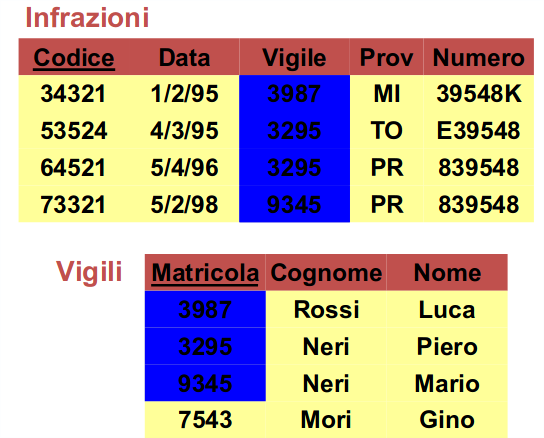
\includegraphics[scale=0.7]{img/infref.png}
	\end{center}
        La definizione precisa e formale richiede un pochino di attenzione in più, in particolare nel caso in
        cui la chiave della relazione riferita sia composta e nel caso in cui vi siano più chiavi, per cui
        procediamo per gradi, incominciando prima con il caso di chiave unica:
        \begin{definizione}
            Sia $R_2$ una relazione con una sola chiave $B$ e sia a sua volta $X = \{A\}$ l'insieme di
            attributi, allora il vincolo di integrità referenziale fra l'attributo $A$ di $R_1$ e la relazione
            $R_2$ risulta soddisfatto se per ogni tupla $t_1$ in $R_1$, in cui $t_1[A]$ non è nullo, esiste una
            tupla $t_2$ in $R_2$ tale che $t_1[A] = t_2[B]$.
        \end{definizione}
        Nel caso più generale bisogna stare attenti al fatto che ogni attributo di $X$ deve corrispondere ad
        uno specifico attributo della chiave primaria di $R_2$ per questo la definizione è la seguente:
        \begin{definizione}
            Siano $X = \{A_1, A_2, \dots, A_n\}$ e $K = \{B_1, B_2, \dots, B_n\}$ due insiemi ordinati di
            attributi per le relazioni $R_1$ e $R_2$, il vincolo risulta soddisfatto se per ogni tupla $t_1$
            in $R_1$, senza attributi nulli su $X$, esiste una tupla $t_2$ in $R_2$ tale per cui $t_1[A_i] =
            t_2[B_i]$, per ogni $i$ compreso tra 1 e p.
        \end{definizione}
        Per analizzare i vincoli di integrità referenziale consideriamo la figura in cui le informazioni 
        della relazione Infrazioni sono rese significative attraverso il collegamento con la relazione Agenti,
        con l'attributo agente, e alla relazione Auto, per mezzo degli attributi stato e numero di targa:
        \begin{center}
        	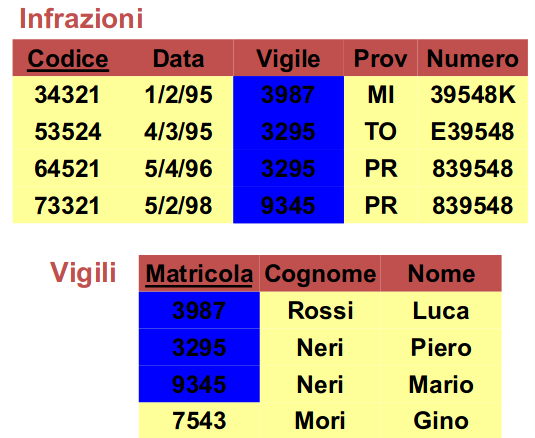
\includegraphics[scale=0.7]{img/inf.png}
        \end{center}
        In questa situazione analizzata abbiamo deciso di inserire i seguenti vincoli referenziali:
        \begin{itemize}
            \item fra l'attributo $Agente$ della relazione Infrarossi e la relazione Agenti.
            \item fra gli attributi Stato e Numero di Infrarossi e la relazione Auto, in cui l'ordine degli
                attributi nella chiave preveda Stato e poi Numero.
        \end{itemize}
        Relativamente al secondo vincolo, notiamo come il ragionamento sull'ordine degli attributi può
        risultare pesante, visto che la corrispondenza può, almeno in questo caso, essere realizzata per mezzo
        dei nomi degli attributi ma in generale ciò non può accedere, quindi l'ordinamento è essenziale.

\end{itemize}

\subsection{In pratica}
Una relazione è spesso rappresentata da una tabella ove le righe rappresentano specifici record e le colonne corrispondono ai campi dei record, l'ordine di righe e colonne è sostanzialmente irrilevante:
\begin{center}
	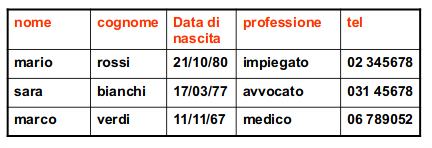
\includegraphics[scale=0.7]{img/rel.png}
\end{center}
\textbf{In una base di dati relazionale ci sono più relazioni:}
\begin{center}
	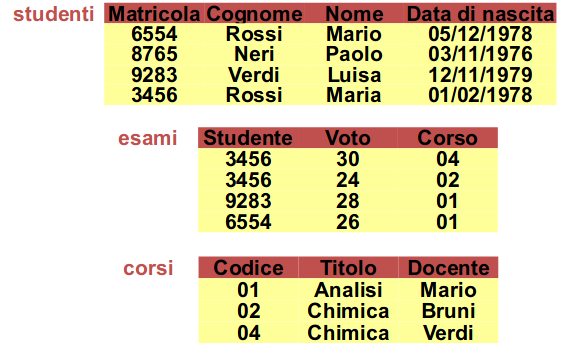
\includegraphics[scale=0.7]{img/rel2.png}
\end{center}
Si hanno 2 componenti:
\begin{enumerate}
	\item lo \textbf{schema}, invariante nel tempo, che ne descrive la struttura(aspetto intensionale). Si rappresenta con le intestazioni delle tabelle
	\item l'\textbf{istanza}, i valori attuali, che possono cambiare anche molto rapidamente (aspetto estensionale). Si rappresenta col corpo di ciascuna tabella
\end{enumerate}
Si hanno 3 accezioni del concetto di relazione:
\begin{enumerate}
	\item \textbf{relazione matematica}: come nella teoria degli insiemi
	\item \textbf{associazione/correlazione} che rappresenta una classe di fatti, nel modello \textit{Entity-Relationship}
	\item \textbf{relazione} secondo il modello relazionale dei dati
\end{enumerate} 
quindi ad esempio:
\begin{center}
	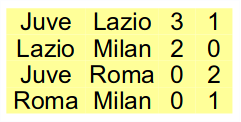
\includegraphics[scale=0.7]{img/mat.png}
\end{center}
\subsection{Relazione Matematica}
Una relazione matematica sugli insiemi $D_1$ e $D_2$, detti \textbf{domini}, è un sottoinsieme del prodotto cartesiano $D_1\times D_2$. Le relazioni si possono visualizzare efficacemente con una tabella in cui ogni colonna corrisponde ad un dominio e ogni riga a un elemento della relazione. Quindi una relazione matematica è un insieme di n-uple ordinate $(d_1,\cdots, d_n) \mbox{ tali che } d_i\in D_i$.\\
Si hanno delle proprietà:
\begin{itemize}
	\item non c'è ordinamento fra le n-uple
	\item le n-uple sono distinte 
	\item ciascuna n-upla è ordinata: l'i-esimo valore proviene dall'i-esimo dominio
\end{itemize}
Dato che ciascuno dei domini ha un ruolo definito dalla posizione nella tabella si ha una \textbf{struttura posizionale}
\subsection{Relazioni nel Modello Relazionale}
Si ha che:
\begin{itemize}
	\item a ciascun dominio si associa un nome (attributo), che  ne descrive il "ruolo"
	\item gli attributi possono essere usati come intestazione
	\item struttura non posizionale
\end{itemize}
Ovvero:
\begin{center}
	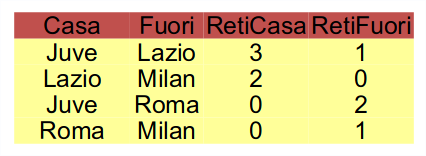
\includegraphics[scale=0.7]{img/rel3.png}
\end{center}
Si hanno delle regole per poter identificare una relazione con una tabella:
\begin{itemize}
	\item i valori di ogni colonna sono fra loro omogenei 
	\item le righe sono diverse fra loro
	\item le intestazioni delle colonne sono diverse tra loro 
\end{itemize}
Inoltre l'ordinamento di righe e colonne è irrilevante.\\
Si possono creare corrispondenze fra le tuple di relazioni distinte per mezzo di valori degli attributi che compaiono nelle ennuple:
\begin{center}
	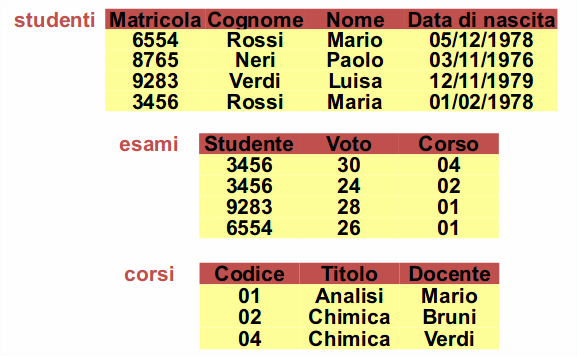
\includegraphics[scale=0.7]{img/rel4.png}
\end{center}
dove matricola e studente rappresentano la stessa informazione, così come corso e codice.\\
Si hanno diversi vantaggi nell'uso della struttura basata su valori:
\begin{itemize}
	\item indipendenza dalle strutture fisiche (si potrebbe avere anche con puntatori di alto livello) che possono cambiare dinamicamente 
	\item si rappresenta solo ciò che è rilevante dal punto di vista dell'applicazione
	\item i dati sono portabili più facilmente da un sistema ad un altro
	\item per accedere ai dati non serve sapere come sono memorizzati fisicamente
\end{itemize}
vediamo quindi un paio di esempi:
\begin{center}
	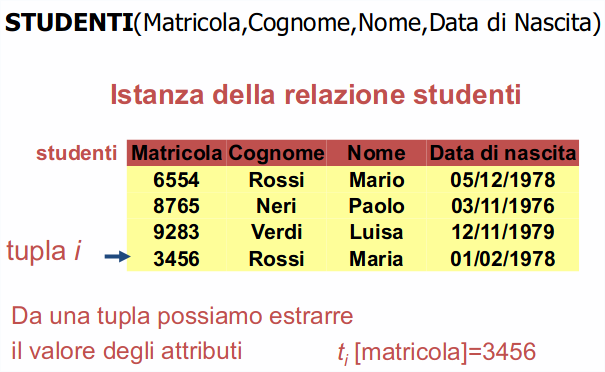
\includegraphics[scale=0.7]{img/rel5.png}
\end{center}
\begin{center}
	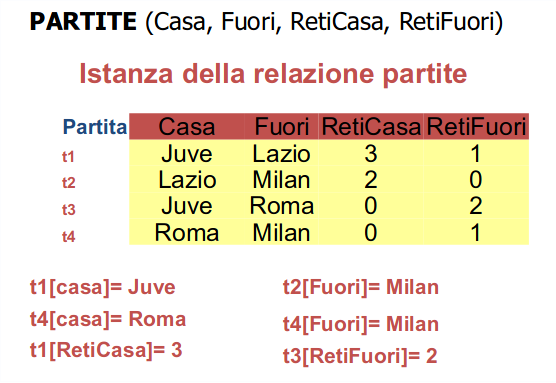
\includegraphics[scale=0.7]{img/rel6.png}
\end{center}
e possono esistere relazioni su  un solo attributo:
\begin{center}
	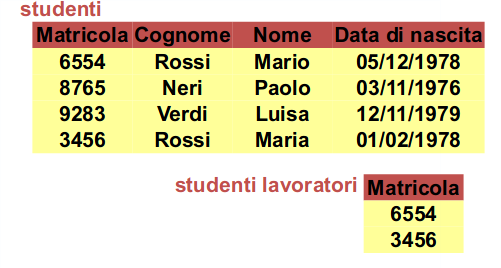
\includegraphics[scale=0.7]{img/rel7.png}
\end{center}
\newpage
Si hanno delle regole di notazione:
\begin{itemize}
	\item \textbf{attributi:} lettere iniziali dell'alfabeto, maiuscole: \textit{A ,B ,C ,A’ ,A1 ,... }
	\item \textbf{insieme di attributi:} lettere finali dell'alfabeto, maiuscole: \textit{X ,Y ,Z ,X’, X1, ...}
	\item \textbf{unioni di insiemi:} $XY$ anziché $X\cup Y$
	\item \textbf{nomi di relazioni:} \textit{R }e lettere circostanti, maiuscole, anche con indici e pedici: \textit{R1, S, S’, ...}
	\item \textbf{relazione:} come il nome della relazione, ma in minuscolo
	\item \textbf{schema di base di dati:} lettera maiuscola in grassetto \textit{\textbf{R}, \textbf{S}, ...}
	\item \textbf{base di dati:} stesso simbolo dello schema, ma in minuscolo
\end{itemize}
Vediamo un'immagine riassuntiva:
\begin{center}
	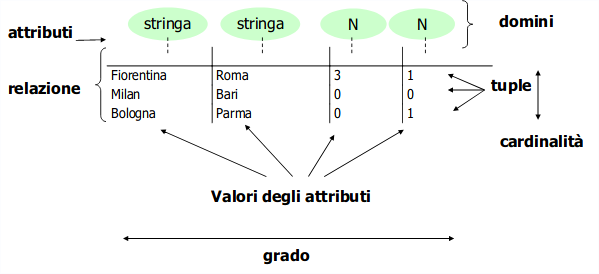
\includegraphics[scale=0.7]{img/ria.png}
\end{center}
Si possono rappresentare strutture nidificate, diverse a seconda della necessità:
\begin{center}
	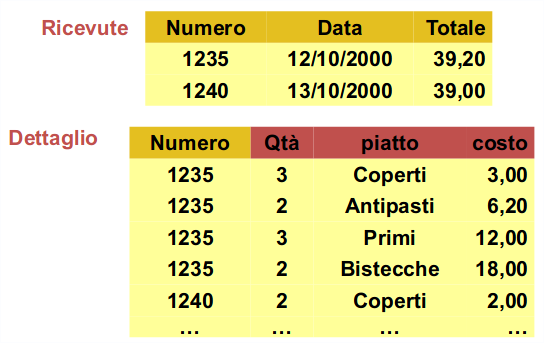
\includegraphics[scale=0.7]{img/rel8.png}
\end{center}
\begin{center}
	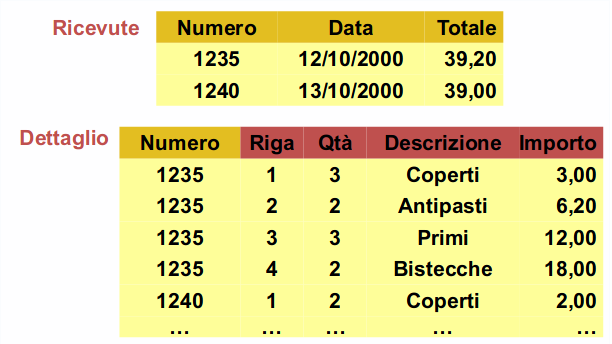
\includegraphics[scale=0.7]{img/rel9.png}
\end{center}
Si definisce la \textbf{chiave} come \textit{l'insieme di attributi che identificano le tuple di una relazione}.\\ Più formalmente un insieme di \textit{K} attributi è una \textbf{superchiave} per \textit{r} se \textit{r} non contiene due tuple distinte $r_1$ e $t_2$ con $t_1[K] = t_2[K]$. Inoltre è chiave per \textit{r} se è una \textbf{superchiave minimale} per \textit{r} (cioè non contiene un'altra superchiave). Vediamo un esempio:
\begin{center}
	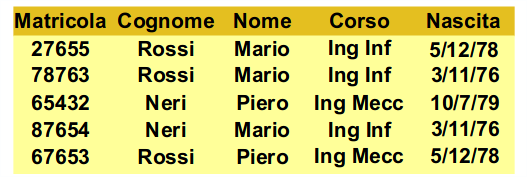
\includegraphics[scale=0.7]{img/rel10.png}
\end{center}
Nella tabella Matricola è una superchiave ed è minimale (contiene un solo attributo). L'insieme dato da Cognome, Nome e Nascita è una superchiave minimale. Volendo sarebbe anche una chiave la coppia Cognome-Corso ma  noi però interessano le chiavi corrispondenti a vincoli di integrità soddisfatti da tutte le relazioni lecite dello schema (sarebbe una chiave senza senso).\\
Il modello relazionale ha una \textbf{struttura rigida}, dove le informazioni sono rappresentate da tuple e solo alcuni formati di tuple sono ammessi (quelli che corrispondono agli schemi di relazione). \textbf{I dati disponibili possono non corrispondere al formato previsto}.\\
Può capitare di avere un'informazione incompleta. In tal caso non conviene usare valori del dominio (0, stringa nulla) perché potrebbero diventare significativi. Si usa quindi il valore nullo \textbf{NULL}, che denota l'assenza di un valore del dominio(e non è un valore del dominio). Si hanno almeno tre casi di valore nullo anche se i DBMS non li distinguono:
\begin{enumerate}
	\item valore sconosciuto 
	\item valore inesistente 
	\item valore senza informazione
\end{enumerate}
Ovviamente l'uso del valore NULL deve essere sensato (per esempio di uno studente non si può avere data di nascita o matricola NULL). Esistono istanze di basi di dati che, pur sintatticamente corrette, non rappresentano informazioni possibili per l'applicazione di interesse. Una chiave in cui non sono ammessi NULL è detta \textbf{chiave primaria} e come notazione si usa la sottolineatura
















\chapter{SQL}
Il linguaggio SQL è un linguaggio per la definizione e la manipolazione dei dati in database relazionali, sviluppato originariamente presso il laboratorio IBM a San Jose’ (California) e adottato nel sistema System R.
L’SQL è stato poi adottato da molti altri DBMS e quindi è stato soggetto ad un’intensa attività di standardizzazione
E‘ un linguaggio con varie funzionalità che contiene:
\begin{itemize}
\item \textbf{DDL:} definizione di domini, tabelle, autorizzazioni, vincoli,
procedure, ecc.
\item \textbf{DML:} linguaggio di query, modifica, ...
\end{itemize}
Si studierà una versione vecchia di SQL in quanto è la più implementata. Nello specifico studieremo SQL-2. SQL-3 è comunque compatibile con SQL-2 e introduce il concetto di oggetto. Noi useremo SQL per definire aggiornare e interrogare la base di dati. Sono sempre più frequenti in realtà sistemi dotati di interfacce più facili da usare. Questi programmi generano le istruzioni SQL corrispondenti.\\
Esistono diverse implementazioni di SQL, per esempio il DBMS di Oracle, Access, Mysql...\\
SQL è relazionale completo e ogni espressione dell'algebra relazionale può essere tradotta in SQL. Il modello dei dati di SQL è basato su tabelle anziché relazioni e possono essere presenti righe duplicate (le tuple) e adotta la logica a 3 valori dell'algebra relazionale (gestendo il null e aggiungendo il valore di verità U, \textit{unknown}). 
\newpage 
Le tabelle di verità diventano quindi:
\begin{center}
	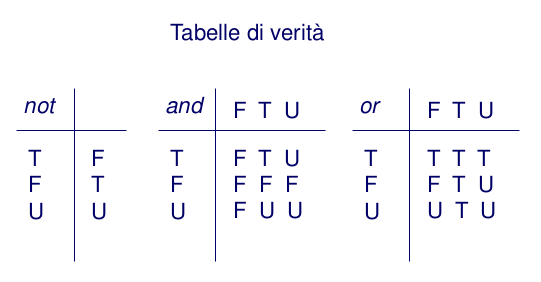
\includegraphics[scale=0.7]{img/unk.png}
\end{center}
Vediamo la notazione per definire la sintassi di SQL:
\begin{itemize}
\item <x> per isolare un termine x
\item $[x]$ indicano che un termine x è opzionale
\item \{x\} indicano che un termine x può essere ripetuto 0
volte o un numero arbitrario di volte
\item | separa opzioni alternative
\end{itemize}
Le parentesi tonde ( ) appartengono al linguaggio
SQL e non alla notazione sopra descritta.\\
Uno \textbf{schema di base di dati} è una collezione di oggetti e ogni schema ha un nome e un proprietario. SI ha la seguente sintassi:
\begin{center}
	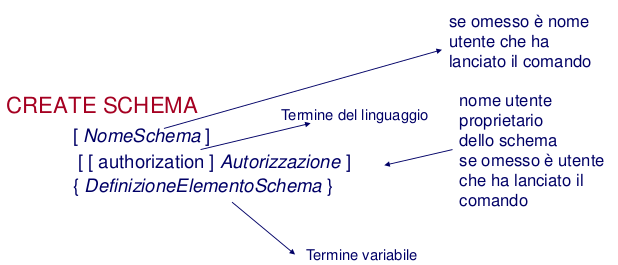
\includegraphics[scale=2.5]{img/sch.png}
\end{center}
Dopo il comando CREATE SCHEMA compaiono le
definizioni dei vari elementi. Non è necessario che la definizione di tutti gli elementi avvenga contemporaneamente alla creazione dello schema. Può avvenire in più fasi successive.\\
Una \textbf{tabella} è costituita da una collezione ordinata
di attributi e da un insieme (eventualmente vuoto) di
vincoli:
\begin{minted}{mysql}
CREATE TABLE NomeTabella (
  NomeAttributo Dominio [ValoreDiDefault] [Vincoli]
  {,NomeAttributo Dominio [ValoreDiDefault] [Vincoli] }
  [AltriVincoli])
\end{minted}
questa istruzione quindi definisce uno schema di relazione e ne crea un'istanza vuota. Per ogni attributo va specificato il dominio, un eventuale valore di default (per questo è comodo il null, che è il valore di default di base) ed eventuali vincoli Possono essere espressi altri vincoli a livello di tabella (tra più attributi).
\\ I \textbf{domini} specificano i valori ammissibili per gli attributi di una relazione. SQL ha 6 domini predefiniti:
\begin{enumerate}
\item bit SQL-2 poi eliminato e sostituito parzialmente da
BOOLEAN in SQL-3
\item carattere
\item numerico Esatto
\item numerico Approssimato
\item data/Ora
\item intervallo Temporale
\end{enumerate}
più ovviamente i domini definiti dall'utente.\\
Vediamo il \textbf{dominio di tipo Bit}. Può essere di lunghezza fissa o variabile. Se la lunghezza non
è specificata corrisponde ad 1 singolo valore.
Corrisponde ad attributi che possono assumere solo due valori
(0,1). Attributi di questo tipo (\textit{flag}) indicano se l'oggetto rappresentato possiede o meno una certa proprietà:
\begin{minted}{mysql}
bit [varying][(lunghezza)]
bit
bit(lunghezza)
bit varying (lunghezza)
varbit (lunghezza)
\end{minted}
\begin{esempio}
Si definisce l'attributo Lavoratore nella relazione STUDENTI per indicare se se lo studente è o meno lavoratore:
\begin{minted}{mysql}
Lavoratore bit
\end{minted}
\end{esempio}
Vediamo il \textbf{tipo carattere}. Rappresenta singoli caratteri alfanumerici oppure stringhe di lunghezza fissa o variabile:
\begin{minted}{mysql}
character [varying] [(lunghezza)]
character o char
character(lunghezza)
varchar(lunghezza)
character varying (lunghezza)
\end{minted}
\begin{esempio}
Si definisce l'attributo Nome della relazione IMPIEGATI come sequenza di caratteri di lunghezza massima 20:
\begin{minted}{mysql}
Nome char(20)
Nome varchar(20)
\end{minted}
con il primo che genera \textit{Paolo\_Bianchi\_ \_ \_ \_ \_ \_ \_} e il secondo \textit{Paolo\_Bianchi}
\end{esempio}
Vediamo i \textbf{tipi numerici esatti}. Rappresentano numeri interi o numeri decimali in virgola fissa (con un
numero prefissato di decimali, ad esempio i valori monetari). Precision è numero di cifre significative, scala il numero di cifre dopo la virgola:
\begin{minted}{mysql}
integer
smallint
numeric numeric(precisione) numeric(precisione,scala)
decimal decimal(precisione) decimal(precisione,scala)
\end{minted}
\begin{esempio}
i definisce l'attributo Eta nella relazione IMPIEGATI:
\begin{minted}{mysql}
Eta decimal(2) // Rappresenta tutti i numeri fra -99 e +99
\end{minted}
Si definisce l'attributo Cambio nella relazione PAGAMENTO per  
il valore del cambio di una certa moneta preciso al centesimo
\begin{minted}{mysql}
Cambio numeric(6,2) // Rappresenta tutti i numeri fra -9999,99 e +9999,99
\end{minted}
\end{esempio}
quindi \textit{INTEGER / SMALLINT} rappresentano valor i interi. La precisione (numero totale di cifre) varia a seconda della specifica
implementazione di SQL, non è specificata nello standard.
SMALLINT richiede minore spazio di memorizzazione.\\
\textit{NUMERIC / DECIMAL} rappresentano i valori decimali.
La differenza tra NUMERIC e DECIMAL è che il primo deve essere implementato esattamente con la precisione richiesta, mentre il secondo può avere una precisione maggiore, la precisione segnalata è requisito minimo. Se la precisione non è specificata si usa il valore caratteristico
dell'implementazione. Per la scala si usa valore 0. Si hanno ovviamente:
\begin{minted}{mysql}
float float(precisione)
double precision
real
\end{minted}
che sono utili per rappresentare valori reali approssimati, ad esempio grandezze fisiche (rappresentazione in virgola mobile, in cui a ciascun numero corrisponde una coppia di valori: mantissa e esponente).\\
Per la data si ha:
\begin{minted}{mysql}
date
time time(precisione)
timestamp timestamp(precisione)
\end{minted}
Ciascuno di questi domini è strutturato e decomponibile in un
insieme di campi (anno, mese, giorno, ora, minuti, secondi):
\begin{minted}{mysql}
DataDiNascita date // 1999-09-18
OraDiConsegna time // 19.24.16
Arrivo timestamp // 2000-09-18 21.15.20
\end{minted}
SI possono avere intervalli temporali:
\begin{minted}{mysql}
interval PrimaUnitàDiTempo
interval PrimaUnitàDiTempo to UltimaUnitàDitempo
\end{minted}
Infine si hanno i tipi \textbf{blob}. Permettono di includere direttamente nel database oggetti molto grandi.
\textit{Binary Large Object (BLOB)} e \textit{Character Large Object (CLOB)}:
\begin{minted}{mysql}
fotografia BLOB(10M)
descrizione CLOB(100k)
\end{minted}
Definiti solo in SQL-3, ma implementati in diversi DBMS
commerciali. Il sistema garantisce solo di memorizzarne il
valore. Non possono essere usati come criterio di selezione
per le interrogazioni.\\
Per creare un dominio uso la primitiva \textit{create domain}:
\begin{minted}{mysql}
CREATE DOMAIN NomeDominio as DominioElementare
             [ValoreDefault] [Constraints]
\end{minted}
Un nuovo dominio è caratterizzato dalle seguenti informazioni:
nome, dominio elementare, valore di default, insieme di vincoli (constraints). Vediamo un esempio:
\begin{minted}{mysql}
CREATE DOMAIN Voto AS SMALLINT
    DEFAULT 0
    NOT NULL
\end{minted}
Il nuovo dominio Voto è definito come uno SMALLINT con
valore di default e che non deve essere null.\\
La definizione di "nuovi domini" è utile perché permette di
associare dei vincoli a un nome di dominio: questo è
importante quando si deve ripetere la stessa definizione di
attributo su diverse tabelle: ad esempio, modifiche alla
definizione di Voto si ripercuotono in tutte le occorrenze di
questo dominio nello schema del Database.
\begin{esempio}
Vediamo un esempio concreto:
\begin{minted}{mysql}
CREATE TABLE NomeTabella (
   NomeAttributo Dominio [ValoreDiDefault] [Vincoli]
   {,NomeAttributo Dominio [ValoreDiDefault] [Vincoli] }
   [AltriVincoli] )

CREATE TABLE Impiegato (
Matricola CHAR(6) PRIMARY KEY,
Nome CHAR(20) NOT NULL,
Cognome CHAR(20) NOT NULL,
Dipart CHAR(15)
Stipendio NUMERIC(9) DEFAULT 0,
UNIQUE (Cognome,Nome)
)
\end{minted}
UNIQUE richiede che non ci siano coppie cognome-nome ripetute
\end{esempio}
Un vincolo (consreaint) è una regola che specifica delle condizioni
sui valori di un elemento dello schema del database.
Un vincolo può essere associato ad una tabella, ad
un attributo, ad un dominio. Sono di due tipi:
\begin{enumerate}
\item \textbf{vincoli intrarelazionali} che si applicano all'interno di una relazione. Possono essere:
\begin{minted}{mysql}
NOT NULL // (Il valore deve essere non nullo)
UNIQUE // (I valori devono essere non ripetuti)
PRIMARY KEY // (Chiave primaria)
CHECK // (Condizioni complesse)
\end{minted}
Il vincolo PRIMARY KEY può essere definito una sola volta
all'interno della relazione. In alcune implementazioni di SQL potrebbe essere
necessario specificare comunque anche il vincolo NOT NULL
per tutti gli attributi coinvolti.
\item \textbf{vincoli interrelazionali} che si applicano tra relazioni diverse. Possono essere definiti attraverso i costrutti sintattici:
\begin{minted}{mysql}
REFERENCES // Permettono di definire vincoli di integrità
FOREIGN KEY // referenziale
CHECK // (Vincoli complessi)
\end{minted}
 e si hanno sintassi per singoli o più attributi. È possibile definire politiche di reazione alle violazioni. Si ha l'\textbf{integrità referenziale} che esprime un legame gerarchico (padre / figlio) fra tabelle. Alcuni attributi della tabella figlio sono definiti
FOREIGN KEY e si devono riferire (REFERENCES)
ad alcuni attributi della tabella padre che costituiscono
una chiave (devono essere UNIQUE e NOT NULL
oppure PRIMARY KEY). I valori contenuti nella FOREIGN KEY devono essere sempre presenti nella tabella padre. SI hanno due sintassi:
\begin{enumerate}
\item nella parte di definizione degli attributi con il
costrutto sintattico REFERENCES:
\begin{minted}{mysql}
AttrFiglio CHAR(3) REFERENCES TabellaPadre(AttrPadre)
\end{minted}
\item oppure dopo le definizioni degli attributi con i
costrutti FOREIGN KEY e REFERENCES:
\begin{minted}{mysql}
FOREIGN KEY (AttrFiglio)
            REFERENCES TabellaPadre(AttrPadre)
\end{minted}
\end{enumerate}
quindi:
\begin{minted}{mysql}
CREATE TABLE Impiegato (
  Matricola CHAR(6) PRIMARY KEY,
  Nome CHAR(20) NOT NULL,
  Cognome CHAR(20) NOT NULL,
  Dipart CHAR(15) REFERENCES Dipartimento(NomeDip) ,
  Stipendio NUMERIC(9) DEFAULT 0,
  UNIQUE (Cognome,Nome)
)
\end{minted}
Se si omettono gli attributi destinazione, vengono
assunti quelli della chiave primaria.
\begin{minted}{mysql}
AttrFiglio CHAR(3) REFERENCES TabellaPadre
\end{minted}
Quando si hanno più attributi da riferire, si utilizza
sempre FOREIGN KEY:
\begin{minted}{mysql}
FOREIGN KEY (AttrFiglio1 {,AttrFiglio2} )
         REFERENCES TabellaPadre(AttrPadre1 {,AttrPadre2})
\end{minted}
\end{enumerate}
\begin{esempio}
Definiamo tre tabelle con le informazioni degli esami
sostenuti dagli studenti: Studente, Esame, Corso:
\begin{minted}{mysql}
CREATE TABLE Studente (
  Matr CHAR(6)
  Nome VARCHAR(30)
  Città VARCHAR(20),
  CDip CHAR(3)
)
\end{minted}
\begin{center}
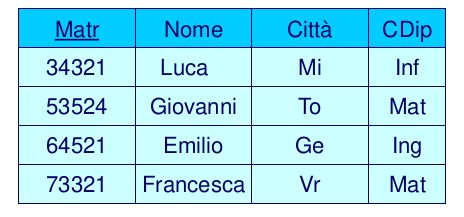
\includegraphics[scale=0.7]{img/st.png}
\end{center}
\begin{minted}{mysql}
CREATE TABLE Esame (
  Matr CHAR(6),
  CodCorso CHAR(6),
  Data DATE NOT NULL,
  Voto Voto,
  PRIMARY KEY (Matr, CodCorso)
\end{minted}
\begin{center}
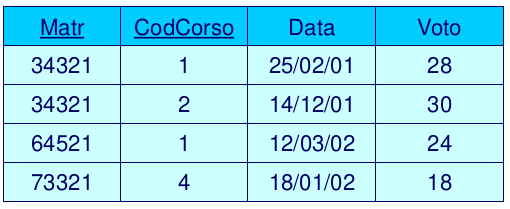
\includegraphics[scale=0.7]{img/es.png}
\end{center}
\begin{minted}{mysql}
  CREATE TABLE Corso (
  CodCorso CHAR(6) PRIMARY KEY,
  Titolo VARCHAR(30) NOT NULL,
  Docente VARCHAR(20)
)
\end{minted}
\begin{center}
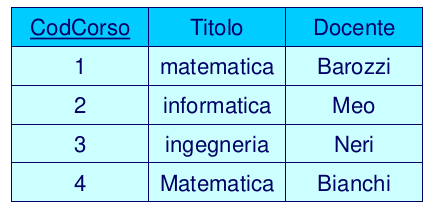
\includegraphics[scale=0.7]{img/sc.png}
\end{center}
con le relazioni:
\begin{center}
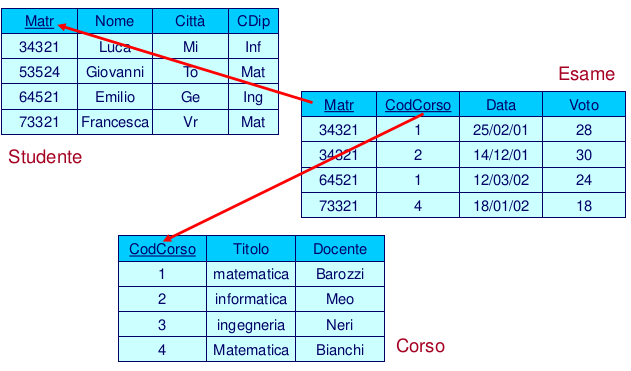
\includegraphics[scale=0.7]{img/re.png}
\end{center}
aggiungiamo un vincolo a esame:
\begin{minted}{mysql}
CREATE TABLE Esame (
  Matr CHAR(6),
  CodCorso CHAR(6),
  Data DATE NOT NULL,
  Voto Voto,
  PRIMARY KEY (Matr, CodCorso)
  FOREIGN KEY (Matr) REFERENCES Studente
  FOREIGN KEY (CodCorso) REFERENCES Corso
\end{minted}
oppure:
\begin{minted}{mysql}
CREATE TABLE Esame (
  Matr CHAR(6), REFERENCES Studente,
  CodCorso CHAR(6),REFERENCES Corso,
  Data DATE NOT NULL,
  Voto Voto,
  PRIMARY KEY (Matr, CodCorso)
\end{minted}
\end{esempio}
Si introduce il \textbf{problema delle violazioni}.\\
Per tutti gli altri vincoli visti fino ad ora, a seguito di
una violazione, il comando di aggiornamento viene
rifiutato segnalando l’errore all’utente.
\\ Per i vincoli di integrità referenziale invece SQL
permette di scegliere delle reazioni da adottare in
caso di violazioni.\\
Si possono introdurre violazioni operando sulle righe della
tabella padre (tabella esterna) o sulle righe della tabella figlio
(tabella interna). Si hanno le seguenti modifiche sulla tabella interna (figlio):
\begin{itemize}
\item inserimento di una nuova riga
\item modefiche della \textit{foreign key}
\end{itemize} 
Inoltre non vengono proposte reazioni, solo il rifiuto dell’operazione\\
Per la tabella esterna (padre) si hanno le seguenti modifiche:
\begin{itemize}
\item cancellazione di una riga
\item modifica dell'attributo riferito
\end{itemize}
inoltre vengono proposte diverse reazioni.\\
Si ha anche il problema dell'aggiornamento. Se rimuovi una matricola alla tabella Esame si aggiunge un problema, il \textbf{problema degli orfani}.\\
Si hanno le reazioni alle violazioni, che si introucono con una modifica (update) dell’attributo cui si fa riferimento o con la cancellazione di tuple. Le reazioni operano sulla tabella figlio (es Esami), in seguito a modifiche alla tabella padre (es Studente):
\begin{minted}{mysql}
CASCADE: propaga la modifica
SET NULL: annulla l’attributo che fa riferimento
SET DEFAULT: assegna il valore di default all’attributo
NO ACTION: impedisce che la modifica possa avvenire
\end{minted}
A fini diagnostici (e di documentazione) è spesso
utile sapere quale vincolo è stato violato a seguito di
un’azione sul DB.
A tale scopo è possibile associare dei nomi ai
vincoli, ad esempio:
\begin{minted}{mysql}
tipendio INTEGER CONSTRAINT StipendioPositivo
CHECK (Stipendio > 0),

CONSTRAINT ForeignKeySedi
FOREIGN KEY (Sede) REFERENCES Sedi
\end{minted}
Per le modiche degli schemi si hanno:
\begin{itemize}
\item ALTER per la modica
\item DROP che cancella oggetti dallo schema
\end{itemize}
\begin{minted}{mysql}
ALTER DOMAIN NomeDominio <
  SET DEFAULT ValoreDefault |
  DROP DEFAULT |
  ADD CONSTRAINT DefVincolo |
  DROP CONSTRAINT NomeVincolo >
  
ALTER TABLE NomeTabella <
  ALTER COLUMN NomeAttributo <
    SET DEFAULT NuovoDefault |
    DROP DEFAULT > |
  DROP COLUMN NomeAttributo |
  ADD COLUMN DefAttributo |
  DROP CONSTRAINT NomeVincolo
  ADD CONSTRAINT DefVincolo >
\end{minted}
DROP cancella oggetti DDL, si applica su domini, tabelle,
indici, view, asserzioni, procedure,..:
\begin{minted}{mysql}
DROP < schema, domain, table, view, ...> NomeElemento
[ RESTRICT | CASCADE ]
\end{minted}
\begin{itemize}
\item RESTRICT: impedisce drop se gli oggetti comprendono istanze
non vuote
\item CASCADE applica drop agli oggetti collegati. Potenziale
pericolosa reazione a catena
\end{itemize}
\subsection{Interrogazioni in SQL}
Le interrogazioni si fanno con la SELECT:
\begin{minted}{mysql}
SELECT ListaAttributi
FROM ListaTabelle
[WHERE Vondizioni] 

SELECT AttrEspr [ [ AS ] Alias ] {, AttrEspr [ [ AS ] Alias ] }
FROM Tabella [ [ AS ] Alias ] {, Tabella [ [ AS ] Alias ] }
[ WHERE Condizione ]
\end{minted} 
con gli AS setto gli alias.
Vediamo qualche esempio:
\begin{minted}{mysql}
-- Individuare lo stipendio degli impiegati di cognome
“Rossi”:
SELECT Stipendio
FROM Impiegato
WHERE Cognome="Rossi"

-- Selezionare nome, cognome e mansione degli
impiegati dell’ufficio 10
SELECT Nome, Cognome, Mansione
FROM Impiegato
WHERE ufficio='10'

-- Individuare le informazioni degli impiegati con
stipendio > 40
Individuare le informazioni degli impiegati con
stipendio > 40

-- Selezionare tutte le informazioni sui dipendenti:
SELECT id_impiegato, Nome, Cognome, Dipart, Ufficio,
stipendio, premioprod,Mansione, Città, idcapo
FROM Impiegato

SELECT *
FROM Impiegato

-- Selezionare cognome, stipendio e premio di
produzione per gli impiegati che hanno uno
stipendio compreso tra 38 e 60:
ELECT cognome, stipendio, premioprod AS premio_di_produzione
FROM Impiegato
WHERE ( stipendio>=38 AND stipendio <=60 )

-- Selezionare i nomi, i cognomi e le città di provenienza
degli impiegati
SELECT Nome, Cognome, città AS città_provenienza
FROM Impiegato

-- Selezionare i nomi e i cognomi degli impiegati, le città
di provenienza e le città in cui lavorano:
SELECT Nome, Cognome, CittàDip AS città_lavoro,
Città AS città_provenienza
FROM Impiegato, Dip
WHERE Dipart = NomeDip

/* Specificare più tabelle su cui operare per determinare il
risultato significa: eseguire il prodotto cartesiano delle tabelle
e poi selezionare le righe che soddisfano clausola WHERE. 
Join di algebra relazionale*/

-- Selezionare i nomi e i cognomi degli impiegati, le città
di provenienza e le città in cui lavorano:
SELECT Nome, Cognome, CittàDip AS città_lavoro,
Città AS città_provenienza
FROM Impiegato, Dip
WHERE Dipart = NomeDip

-- Selezionare i nomi e i cognomi degli impiegati, le città
di provenienza e le città in cui lavorano:
SELECT Nome, Cognome, Città AS città_lavoro,
Città AS città_provenienza
FROM Impiegato, Dip
WHERE Dipart = Nome

/* Notazione punto: si utilizza il nome della tabella cui
l’attributo fa riferimento */
SELECT Impiegato.Nome, Cognome, Dip.Città AS città_lavoro,
Impiegato.Città AS città_provenienza
FROM Impiegato, Dip
WHERE Dipart = Dip.Nome

/* Si usano Alias per ridenominare le tabelle:
1) Abbreviano riferimento a tabelle
2) Risolvono ambiguità di riferimento*/
SELECT I.Nome, Cognome, D.Città AS città_lavoro,
I.Città AS città_provenienza
FROM Impiegato I, Dip D
WHERE Dipart = D.Nome
\end{minted}
\textbf{pagina 18}


\section{Progettazione Concettuale, approfondimento}
La \textbf{progettazione concettuale} di una base di dati consiste nella costruzione di uno
schema\textbf{ Entità-Relazione} in grado di descrivere al meglio le specifiche sui dati di
una applicazione. Anche nel caso di applicazioni non particolarmente complesse,
lo schema che si ottiene può contenere molti concetti correlati in una maniera
piuttosto complicata. Ne consegue che la costruzione dello schema finale è, necessariamente,
un processo graduale: lo schema concettuale viene progressivamente
raffinato e arricchito attraverso una serie di trasformazioni ed eventuali correzioni.
In questo capitolo verranno descritte le strategie che è possibile seguire in questo
processo di sviluppo di uno schema concettuale.
\\Per \textbf{raccolta dei requisiti} si intende la completa individuazione dei problemi
che l'applicazione da realizzare deve risolvere, con le proprie caratteristuche
Per \textbf{caratteristiche dei sistema} si intendono sia gli aspetti \textit{statici}, ovvero di \textbf{dati}, che quelli \textit{dinamici}, ovvero le \textbf{operazioni sui dati}. I requisiti vengono innanzitutto raccolti in specifiche espresse in linguaggio naturale per questo motivo, spesso ambigue e disorganizzate.\\
L'analisi dei requisiti consiste nel chiarimento e nell'organizzazione delle specifiche dei requisiti. Si tratta
ovviamente di attività fortemente interconnesse: l'attività di analisi inizia con i
primi requisiti ottenuti per poi procedere di pari passo con l'attività di raccolta.
In molti casi è l'attività stessa di analisi dei requisiti che suggerisce successive
attività di raccolta.\\
I requisiti provengono da vari tipi di fonte:
\begin{itemize}
\item \textbf{utenti dell'applicazione}
\item \textbf{documentazione pre-esistente}
\item \textbf{implementazione pre-esistente}
\end{itemize}
Risulta chiaro che, nella fase di acquisizione delle specifiche, gioca un importante ruolo l'interazione con gli utenti del sistema informativo.\\
Come criterio generale da seguire possiamo dire che, nel corso delle intervi-
ste, è opportuno effettuare con l'utente verifiche di comprensione e consistenza
sulle informazioni che si stanno raccogliendo. Questo può essere fatto attraverso
esempi (generali e relativi a casi limite) oppure richiedendo definizioni e classificazioni precise. E inoltre molto importante in questa fase cercare di individuare
gli aspetti essenziali rispetto a quelli marginali e procedere per raffinamenti successivi. Partendo quindi dai principali aspetti del problema allo studio, dei quali
si ha inizialmente una conoscenza solo parziale, si procede cercando di acquisire
via via maggiori dettagli.\\
Sappiamo bene però che il linguaggio naturale è fonte di ambiguità e frainten-
dimenti. E molto importante quindi effettuare una profonda analisi del testo che
descrive le specifiche per filtrare le eventuali inesattezze e i termini ambigui presenti.\\
Proviamo a fissare alcune regole generali per ottenere una specifica dei requi-
siti più precisa e senza ambiguità:
\begin{itemize}
\item \textbf{scegliere il corretto livello di astrazione}, evitando di utilizzare termini
  troppo generici o troppo specifici che rendono poco chiaro un concetto
\item \textbf{standardizzare la struttura delle frasi}, utilizzando sempre lo stesso stile sintattico
\item \textbf{evitare frasi contorte}, preferendo semplicità e chiarezza
\item \textbf{individuare sinonimi/omonimi e unificare i termini}, per evitare ambiguità
\item \textbf{rendere esplicito il riferimento tra termini}, infatti può
  succedere che l'assenza di un contesto di riferimento renda alcuni concetti
  ambigui: in questi casi bisogna esplicitare il riferimento tra termini.
  In questo caso si deve esplicitare chiaramente a chi ci si sta riferendo,
  per evitare confusione
  \newpage
\item \textbf{costruire un glossario dei termini}, infatti è molto utile, per la comprensione e la
  precisazione dei termini usati, definire un glossario che, per ogni termine,
  contenga: una breve descrizione, possibili sinonimi e altri termini contenuti nel
  glossario con i quali esiste un legame logico. Vediamo un esempio pratico:
  \begin{center}
    \includegraphics[scale=0.7]{img/glo.png}
  \end{center}
\end{itemize}
\textbf{Dopo aver individuato le varie ambiguità e le imprecisioni, esse vanno eliminate
sostituendo i termini non corretti con termini più adeguati. In caso di dubbio, è
necessario intervistare nuovamente colui che ha fornito il dato o consultare la
documentazione relativa.}\\
A questo punto possiamo riscrivere le nostre specifiche apportando le modi-
fiche proposte. È molto utile, in questa fase, decomporre il testo in gruppi di frasi
omogenee, relative cioè agli stessi concetti. Naturalmente, accanto alle specifiche sui dati, vanno raccolte le specifiche
sulle operazioni da effettuare su questi dati. Bisogna cercare di utilizzare la me-
desima terminologia usata per i dati (possiamo per questo far riferimento al glos-
sario dei termini) e informarci anche sulla frequenza con la quale le varie operazioni vengono eseguite. Come vedremo, la conoscenza di questa informazione
sarà determinante nella fase di progettazione logica.

\chapter{Progettazione Logica}
L'obiettivo della progettazione \textbf{logic}a è quello di costruire uno schema logico in
grado di descrivere, in maniera corretta ed efficiente, tutte le informazioni
contenute nello schema Entità-Relazione prodotto nella fase di progettazione concettuale. Si hanno due necessità:
\begin{enumerate}
\item "semplificare" la traduzione
\item "ottimizzare" il progetto
\end{enumerate}
La semplificazione dello schema si rende necessaria perché non tutti i costrutti
del modello Entità-Relazione hanno una traduzione naturale nei modelli logici,
vedisi la generalizzazione.\\
Inoltre, mentre la progettazione concettuale ha come obiettivo la rappresentazione
accurata e naturale dei dati d'interesse dal punto di vista del significato che hanno nell'applicazione,
la progettazione logica costituisce la base per l'effettiva realizzazione dell'applicazione
e deve tenere conto, per quanto possibile, delle sue
prestazioni: questa necessità può portare a una ristrutturazione dello schema concettuale
che renda più efficiente l'esecuzione delle operazioni previste.
Pertanto, è necessario prevedere sia un'attività di \textbf{riorganizzazion}e,
sia un'attività di \textbf{traduzione} (dal modello concettuale a quello logico). Nel resto di questo capitolo, dopo
un breve inquadramento metodologico, presenteremo separatamente queste due
attività.
\newpage
Si hanno due fasi principali nella programmazione logica:
\begin{enumerate}
\item \textbf{ristrutturazione dello schema E-R}, che è una fase indipendente dal
modello logico scelto e si basa su criteri di ottimizzazione dello schema e di
semplificazione della fase successiva
\item \textbf{traduzione verso il modello logico}, che fa riferimento a uno specifico modello logivo (come il modello relazionale) è può includere una ulteriore ottimizzazione che si basa sulle caratteristiche del modello logico stesso
\end{enumerate}
\begin{center}
\includegraphics[scale=0.9]{img/log.png}
\end{center}
I dati di ingresso della prima fase sono lo schema concettuale prodotto nella fa-
se precedente e il carico applicativo previsto, in termini di dimensione dei dati
e caratteristiche delle operazioni. Il risultato che si ottiene è uno schema E-R ristrutturato, che non è più uno schema concettuale nel senso stretto del termine,
in quanto costituisce una rappresentazione dei dati che tiene conto degli aspetti
realizzativi. Questo schema e il modello logico scelto costituiscono i dati di ingresso
della seconda fase, che produce lo schema logico della nostra base di dati.
In questa seconda fase è possibile effettuare verifiche della qualità dello schema ed
eventuali ulteriori ottimizzazioni mediante tecniche basate sulle caratteristiche del
modello logico. Si parlerà in seguito della normalizzazione. Lo schema logico finale,
i vincoli di integrità definiti su di esso e la relativa documentazione, costituiscono
i prodotti finali della progettazione logica.
\section{Analisi dell'E-R}
Abbiamo detto che uno schema E-R può essere modificato per ottimizzare alcu-
ni indici di prestazione del progetto. Parliamo di indici di prestazione e non di
prestazioni perché, in realtà, le prestazioni di una base di dati non sono valutabili
in maniera precisa in sede di progettazione logica, in quanto dipendenti anche da
parametri fisici: dal sistema di gestione di basi di dati che verrà utilizzato e da
altri fattori difficilmente prevedibili in questa fase.
\\Si possono comunque studiare due fattori che regolano anche le prestazioni dei sistemi software:
\begin{enumerate}
\item \textbf{costo di un'operazione}, ovvero viene valutato in termini di numero di occorrenze
di entità e associazioni che mediamente vanno visitate per rispondere a una
operazione sulla base di dati; questa schematizzazione è molto forte e sarà
talvolta nessesrio riferirsi a un criterio più fine
\item \textbf{occupazione della memoria}, ovvero viene valutato in termini dello spazio di memoria
(misurato per esempio in numero di byte) necessario per memorizzare i dati
descritti dallo schema
\end{enumerate}
Oltre allo schema si necessiterà anche di:
\begin{itemize}
\item \textbf{volume dei dati}, ovvero il numero di occorrenze di ogni entità e associazione
  dello schema e la dimensione di qualsiasi attributo, sia di relazione che di associazione
\item \textbf{caratteristiche delle operazioni}, ovvero il tipo dell'operazione,
  la frequenza (ovvero il numero medio di esecuzioni in un intervallo di tempo)
  della stessa e i dati coinvolti, che asiano associazioni e/o entità
\end{itemize}
Si ha la cosiddetta \textbf{ottanta-venti} in base alla quale l'80\% del carico è generato dal 20\%  delle operazioni.\\
Il volume dei dati e le caratteristiche generali delle operazioni possono essere
descritti facendo uso di tabelle. Nella tavola dei volumi
vengono riportati tutti i concetti dello schema (entità e associazioni) con il volume previsto a regime. Nella tavola delle operazioni riportiamo, per ogni operazione,
la frequenza prevista e un simbolo che indica se l'operazione è interattiva (1) o
batch (B). Nella tavola dei volumi, il numero delle occorrenze delle associazioni
dipende da due parametri: il numero di occorrenze delle entità coinvolte nelle as
sociazioni e il numero (medio) di partecipazioni di una occorrenza di entità alle
occorrenze di associazioni. 11 secondo parametro dipende a sua volta dalle cardi-
nalità delle associazioni. Vediamo un esempio:
\begin{center}
\includegraphics[scale=0.9]{img/tav.png}
\end{center}
Per ogni operazione, possiamo inoltre descrivere graficamente i dati coinvolti
con uno schema di operazione che consiste nel frammento dello schema E-R
interessato dall'operazione, sul quale viene disegnato il "cammino logico" da
percorrere per accedere alle informazioni d'interesse. Si ha quindi un esempio
di \textbf{schema di operazione:}
\begin{center}
\includegraphics[scale=0.9]{img/opt.png}
\end{center}
Si ha poi la \textbf{tavola degli accessi}, che presenta nell'ul-
tima colonna di questa tabella viene riportato il tipo di accesso: L per accesso in
lettura e S per accesso in scrittura. Questa distinzione va fatta perché, generalmente, le operazioni di scrittura sono più onerose di quelle in lettura (in quanto
devono essere eseguite in modo esclusivo e possono richiedere l'aggiornamento di
indici, che sono strutture ausiliarie per l'accesso efficiente ai dati): Vediamo un esempio:
\begin{center}
\includegraphics[scale=1]{img/ac.png}
\end{center}
\newpage
\subsection{Ristrutturazione dell'E-R}
La fase di ristrutturazione di uno schema Entità-Relazione si può suddividere in
una serie di passi da effettuare in sequenza:
\begin{enumerate}
\item \textbf{analisi delle ridondanze}, dove si decide se eliminare o mantenere eventuali ridondanze presenti nello schema
\item \textbf{eliminazione delle generalizzazioni}, dove tutte le generalizzazioni presenti nello
  schema vengono analizzate e sostituite da altri costrutti
\item \textbf{partizionamento/accorpamento di entità e associazioni}, dove si decide
  se è opportuno partizionare concetti dello schema (entità e/o associazioni) in più
  concetti o, viceversa, accorpare concetti separati in un unico concetto
\item \textbf{scelta degli identificatori principali}, dove si seleziona un identificatore per quelle entità che ne hanno più di uno
\end{enumerate}
Si ha quindi:
\begin{center}
\includegraphics[scale=0.8]{img/rer.png}
\end{center}
\newpage
\subsubsection{Analisi delle Ridondanze}
Ricordiamo che una ridondanza in uno schema concettuale corrisponde alla pre-
senza di un dato che può essere derivato (cioè ottenuto attraverso una serie di operazioni) da altri dati. In particolare, in uno schema Entità-Relazione si possono
presentare varie forme di ridondanza.
Si hanno dei casi frequenti:
\begin{itemize}
\item attributi derivabili, occorrenza per occorrenza, da altri attributi della stessa entità o associazione
\item attributi derivabili da attributi di altre entità (o associazioni), di solito attraverso
funzioni aggregative
\end{itemize}
Vediamo qualche esempio di schemi con ridondanze:
\begin{center}
\includegraphics[scale=1]{img/rid.png}
\end{center}
\newpage
La presenza di un dato derivato presenta un vantaggio e alcuni svantaggi. 11 van-
taggio è una riduzione degli accessi necessari per calcolare il dato derivato,
gli svantaggi sono una maggiore occupazione di memoria (che è comunque spesso un
costo trascurabile) e la necessità di effettuare operazioni aggiuntive per mantenere
il dato derivato aggiornato. La decisione di mantenere o eliminare una ridondanza
va quindi presa confrontando costo di esecuzione delle operazioni che coinvolgono
il dato ridondante e relativa occupazione di memoria, nei casi di presenza e
assenza della ridondanza. Vediamo come cambiano le tavole degli accessi:
\begin{center}
\includegraphics[scale=1]{img/rid2.png}
\end{center}
%pagina 311
\end{document}



